
%% bare_conf.tex
%% V1.3
%% 2007/01/11
%% by Michael Shell
%% See:
%% http://www.michaelshell.org/
%% for current contact information.
%%
%% This is a skeleton file demonstrating the use of IEEEtran.cls
%% (requires IEEEtran.cls version 1.7 or later) with an IEEE conference paper.
%%
%% Support sites:
%% http://www.michaelshell.org/tex/ieeetran/
%% http://www.ctan.org/tex-archive/macros/latex/contrib/IEEEtran/
%% and
%% http://www.ieee.org/

%%*************************************************************************
%% Legal Notice:
%% This code is offered as-is without any warranty either expressed or
%% implied; without even the implied warranty of MERCHANTABILITY or
%% FITNESS FOR A PARTICULAR PURPOSE! 
%% User assumes all risk.
%% In no event shall IEEE or any contributor to this code be liable for
%% any damages or losses, including, but not limited to, incidental,
%% consequential, or any other damages, resulting from the use or misuse
%% of any information contained here.
%%
%% All comments are the opinions of their respective authors and are not
%% necessarily endorsed by the IEEE.
%%
%% This work is distributed under the LaTeX Project Public License (LPPL)
%% ( http://www.latex-project.org/ ) version 1.3, and may be freely used,
%% distributed and modified. A copy of the LPPL, version 1.3, is included
%% in the base LaTeX documentation of all distributions of LaTeX released
%% 2003/12/01 or later.
%% Retain all contribution notices and credits.
%% ** Modified files should be clearly indicated as such, including  **
%% ** renaming them and changing author support contact information. **
%%
%% File list of work: IEEEtran.cls, IEEEtran_HOWTO.pdf, bare_adv.tex,
%%                    bare_conf.tex, bare_jrnl.tex, bare_jrnl_compsoc.tex
%%*************************************************************************

% *** Authors should verify (and, if needed, correct) their LaTeX system  ***
% *** with the testflow diagnostic prior to trusting their LaTeX platform ***
% *** with production work. IEEE's font choices can trigger bugs that do  ***
% *** not appear when using other class files.                            ***
% The testflow support page is at:
% http://www.michaelshell.org/tex/testflow/



% Note that the a4paper option is mainly intended so that authors in
% countries using A4 can easily print to A4 and see how their papers will
% look in print - the typesetting of the document will not typically be
% affected with changes in paper size (but the bottom and side margins will).
% Use the testflow package mentioned above to verify correct handling of
% both paper sizes by the user's LaTeX system.
%
% Also note that the "draftcls" or "draftclsnofoot", not "draft", option
% should be used if it is desired that the figures are to be displayed in
% draft mode.
%
\documentclass[10pt, conference, compsocconf]{IEEEtran}
% Add the compsocconf option for Computer Society conferences.
%
% If IEEEtran.cls has not been installed into the LaTeX system files,
% manually specify the path to it like:
% \documentclass[conference]{../sty/IEEEtran}





% Some very useful LaTeX packages include:
% (uncomment the ones you want to load)


% *** MISC UTILITY PACKAGES ***
%
%\usepackage{ifpdf}
% Heiko Oberdiek's ifpdf.sty is very useful if you need conditional
% compilation based on whether the output is pdf or dvi.
% usage:
% \ifpdf
%   % pdf code
% \else
%   % dvi code
% \fi
% The latest version of ifpdf.sty can be obtained from:
% http://www.ctan.org/tex-archive/macros/latex/contrib/oberdiek/
% Also, note that IEEEtran.cls V1.7 and later provides a builtin
% \ifCLASSINFOpdf conditional that works the same way.
% When switching from latex to pdflatex and vice-versa, the compiler may
% have to be run twice to clear warning/error messages.






% *** CITATION PACKAGES ***
%
%\usepackage{cite}
% cite.sty was written by Donald Arseneau
% V1.6 and later of IEEEtran pre-defines the format of the cite.sty package
% \cite{} output to follow that of IEEE. Loading the cite package will
% result in citation numbers being automatically sorted and properly
% "compressed/ranged". e.g., [1], [9], [2], [7], [5], [6] without using
% cite.sty will become [1], [2], [5]--[7], [9] using cite.sty. cite.sty's
% \cite will automatically add leading space, if needed. Use cite.sty's
% noadjust option (cite.sty V3.8 and later) if you want to turn this off.
% cite.sty is already installed on most LaTeX systems. Be sure and use
% version 4.0 (2003-05-27) and later if using hyperref.sty. cite.sty does
% not currently provide for hyperlinked citations.
% The latest version can be obtained at:
% http://www.ctan.org/tex-archive/macros/latex/contrib/cite/
% The documentation is contained in the cite.sty file itself.






% *** GRAPHICS RELATED PACKAGES ***
%
\ifCLASSINFOpdf
   \usepackage[pdftex]{graphicx}
  % declare the path(s) where your graphic files are
  % \graphicspath{{../pdf/}{../jpeg/}}
  % and their extensions so you won't have to specify these with
  % every instance of \includegraphics
  % \DeclareGraphicsExtensions{.pdf,.jpeg,.png}
\else
  % or other class option (dvipsone, dvipdf, if not using dvips). graphicx
  % will default to the driver specified in the system graphics.cfg if no
  % driver is specified.
  % \usepackage[dvips]{graphicx}
  % declare the path(s) where your graphic files are
  % \graphicspath{{../eps/}}
  % and their extensions so you won't have to specify these with
  % every instance of \includegraphics
  % \DeclareGraphicsExtensions{.eps}
\fi
% graphicx was written by David Carlisle and Sebastian Rahtz. It is
% required if you want graphics, photos, etc. graphicx.sty is already
% installed on most LaTeX systems. The latest version and documentation can
% be obtained at: 
% http://www.ctan.org/tex-archive/macros/latex/required/graphics/
% Another good source of documentation is "Using Imported Graphics in
% LaTeX2e" by Keith Reckdahl which can be found as epslatex.ps or
% epslatex.pdf at: http://www.ctan.org/tex-archive/info/
%
% latex, and pdflatex in dvi mode, support graphics in encapsulated
% postscript (.eps) format. pdflatex in pdf mode supports graphics
% in .pdf, .jpeg, .png and .mps (metapost) formats. Users should ensure
% that all non-photo figures use a vector format (.eps, .pdf, .mps) and
% not a bitmapped formats (.jpeg, .png). IEEE frowns on bitmapped formats
% which can result in "jaggedy"/blurry rendering of lines and letters as
% well as large increases in file sizes.
%
% You can find documentation about the pdfTeX application at:
% http://www.tug.org/applications/pdftex





% *** MATH PACKAGES ***
%
%\usepackage[cmex10]{amsmath}
% A popular package from the American Mathematical Society that provides
% many useful and powerful commands for dealing with mathematics. If using
% it, be sure to load this package with the cmex10 option to ensure that
% only type 1 fonts will utilized at all point sizes. Without this option,
% it is possible that some math symbols, particularly those within
% footnotes, will be rendered in bitmap form which will result in a
% document that can not be IEEE Xplore compliant!
%
% Also, note that the amsmath package sets \interdisplaylinepenalty to 10000
% thus preventing page breaks from occurring within multiline equations. Use:
%\interdisplaylinepenalty=2500
% after loading amsmath to restore such page breaks as IEEEtran.cls normally
% does. amsmath.sty is already installed on most LaTeX systems. The latest
% version and documentation can be obtained at:
% http://www.ctan.org/tex-archive/macros/latex/required/amslatex/math/





% *** SPECIALIZED LIST PACKAGES ***
%
%\usepackage{algorithmic}
% algorithmic.sty was written by Peter Williams and Rogerio Brito.
% This package provides an algorithmic environment fo describing algorithms.
% You can use the algorithmic environment in-text or within a figure
% environment to provide for a floating algorithm. Do NOT use the algorithm
% floating environment provided by algorithm.sty (by the same authors) or
% algorithm2e.sty (by Christophe Fiorio) as IEEE does not use dedicated
% algorithm float types and packages that provide these will not provide
% correct IEEE style captions. The latest version and documentation of
% algorithmic.sty can be obtained at:
% http://www.ctan.org/tex-archive/macros/latex/contrib/algorithms/
% There is also a support site at:
% http://algorithms.berlios.de/index.html
% Also of interest may be the (relatively newer and more customizable)
% algorithmicx.sty package by Szasz Janos:
% http://www.ctan.org/tex-archive/macros/latex/contrib/algorithmicx/




% *** ALIGNMENT PACKAGES ***
%
%\usepackage{array}
% Frank Mittelbach's and David Carlisle's array.sty patches and improves
% the standard LaTeX2e array and tabular environments to provide better
% appearance and additional user controls. As the default LaTeX2e table
% generation code is lacking to the point of almost being broken with
% respect to the quality of the end results, all users are strongly
% advised to use an enhanced (at the very least that provided by array.sty)
% set of table tools. array.sty is already installed on most systems. The
% latest version and documentation can be obtained at:
% http://www.ctan.org/tex-archive/macros/latex/required/tools/


%\usepackage{mdwmath}
%\usepackage{mdwtab}
% Also highly recommended is Mark Wooding's extremely powerful MDW tools,
% especially mdwmath.sty and mdwtab.sty which are used to format equations
% and tables, respectively. The MDWtools set is already installed on most
% LaTeX systems. The lastest version and documentation is available at:
% http://www.ctan.org/tex-archive/macros/latex/contrib/mdwtools/


% IEEEtran contains the IEEEeqnarray family of commands that can be used to
% generate multiline equations as well as matrices, tables, etc., of high
% quality.


%\usepackage{eqparbox}
% Also of notable interest is Scott Pakin's eqparbox package for creating
% (automatically sized) equal width boxes - aka "natural width parboxes".
% Available at:
% http://www.ctan.org/tex-archive/macros/latex/contrib/eqparbox/





% *** SUBFIGURE PACKAGES ***
%\usepackage[tight,footnotesize]{subfigure}
% subfigure.sty was written by Steven Douglas Cochran. This package makes it
% easy to put subfigures in your figures. e.g., "Figure 1a and 1b". For IEEE
% work, it is a good idea to load it with the tight package option to reduce
% the amount of white space around the subfigures. subfigure.sty is already
% installed on most LaTeX systems. The latest version and documentation can
% be obtained at:
% http://www.ctan.org/tex-archive/obsolete/macros/latex/contrib/subfigure/
% subfigure.sty has been superceeded by subfig.sty.



%\usepackage[caption=false]{caption}
%\usepackage[font=footnotesize]{subfig}
% subfig.sty, also written by Steven Douglas Cochran, is the modern
% replacement for subfigure.sty. However, subfig.sty requires and
% automatically loads Axel Sommerfeldt's caption.sty which will override
% IEEEtran.cls handling of captions and this will result in nonIEEE style
% figure/table captions. To prevent this problem, be sure and preload
% caption.sty with its "caption=false" package option. This is will preserve
% IEEEtran.cls handing of captions. Version 1.3 (2005/06/28) and later 
% (recommended due to many improvements over 1.2) of subfig.sty supports
% the caption=false option directly:
%\usepackage[caption=false,font=footnotesize]{subfig}
%
% The latest version and documentation can be obtained at:
% http://www.ctan.org/tex-archive/macros/latex/contrib/subfig/
% The latest version and documentation of caption.sty can be obtained at:
% http://www.ctan.org/tex-archive/macros/latex/contrib/caption/




% *** FLOAT PACKAGES ***
%
%\usepackage{fixltx2e}
% fixltx2e, the successor to the earlier fix2col.sty, was written by
% Frank Mittelbach and David Carlisle. This package corrects a few problems
% in the LaTeX2e kernel, the most notable of which is that in current
% LaTeX2e releases, the ordering of single and double column floats is not
% guaranteed to be preserved. Thus, an unpatched LaTeX2e can allow a
% single column figure to be placed prior to an earlier double column
% figure. The latest version and documentation can be found at:
% http://www.ctan.org/tex-archive/macros/latex/base/



%\usepackage{stfloats}
% stfloats.sty was written by Sigitas Tolusis. This package gives LaTeX2e
% the ability to do double column floats at the bottom of the page as well
% as the top. (e.g., "\begin{figure*}[!b]" is not normally possible in
% LaTeX2e). It also provides a command:
%\fnbelowfloat
% to enable the placement of footnotes below bottom floats (the standard
% LaTeX2e kernel puts them above bottom floats). This is an invasive package
% which rewrites many portions of the LaTeX2e float routines. It may not work
% with other packages that modify the LaTeX2e float routines. The latest
% version and documentation can be obtained at:
% http://www.ctan.org/tex-archive/macros/latex/contrib/sttools/
% Documentation is contained in the stfloats.sty comments as well as in the
% presfull.pdf file. Do not use the stfloats baselinefloat ability as IEEE
% does not allow \baselineskip to stretch. Authors submitting work to the
% IEEE should note that IEEE rarely uses double column equations and
% that authors should try to avoid such use. Do not be tempted to use the
% cuted.sty or midfloat.sty packages (also by Sigitas Tolusis) as IEEE does
% not format its papers in such ways.





% *** PDF, URL AND HYPERLINK PACKAGES ***
%
%\usepackage{url}
% url.sty was written by Donald Arseneau. It provides better support for
% handling and breaking URLs. url.sty is already installed on most LaTeX
% systems. The latest version can be obtained at:
% http://www.ctan.org/tex-archive/macros/latex/contrib/misc/
% Read the url.sty source comments for usage information. Basically,
% \url{my_url_here}.

\usepackage{paralist}
\usepackage{caption}
\usepackage{subcaption}



% *** Do not adjust lengths that control margins, column widths, etc. ***
% *** Do not use packages that alter fonts (such as pslatex).         ***
% There should be no need to do such things with IEEEtran.cls V1.6 and later.
% (Unless specifically asked to do so by the journal or conference you plan
% to submit to, of course. )


% correct bad hyphenation here
\hyphenation{op-tical net-works semi-conduc-tor}


\begin{document}
%
% paper title
% can use linebreaks \\ within to get better formatting as desired
\title{Evaluating Different Distributed-Cyber-Infrastructure for Data and Compute Intensive Scientific Application}


% author names and affiliations
% use a multiple column layout for up to two different
% affiliations

\author{\IEEEauthorblockN{Arghya Kusum Das, Seung-Jong Park}
\IEEEauthorblockA{School of Electrical Engineering and Computer Science\\
Center for Computation and Technology\\
Louisiana State University, Baton Rouge, LA, 70803 \\
Email: \{adas7, sjpark\} @lsu.edu}
\and
\IEEEauthorblockN{Jaeki Hong, Wooseok Chang}
\IEEEauthorblockA{Samsung Electronics Co., Ltd.\\
95, Samsung 2-ro\\
Giheung-gu, Yongin-si, Gyeonggi-do, 446711\\
Email: \{jaeki.hong, wooseok\_chang\} @samsung.com}
}

% conference papers do not typically use \thanks and this command
% is locked out in conference mode. If really needed, such as for
% the acknowledgment of grants, issue a \IEEEoverridecommandlockouts
% after \documentclass

% for over three affiliations, or if they all won't fit within the width
% of the page, use this alternative format:
% 
%\author{\IEEEauthorblockN{Michael Shell\IEEEauthorrefmark{1},
%Homer Simpson\IEEEauthorrefmark{2},
%James Kirk\IEEEauthorrefmark{3}, 
%Montgomery Scott\IEEEauthorrefmark{3} and
%Eldon Tyrell\IEEEauthorrefmark{4}}
%\IEEEauthorblockA{\IEEEauthorrefmark{1}School of Electrical and Computer Engineering\\
%Georgia Institute of Technology,
%Atlanta, Georgia 30332--0250\\ Email: see http://www.michaelshell.org/contact.html}
%\IEEEauthorblockA{\IEEEauthorrefmark{2}Twentieth Century Fox, Springfield, USA\\
%Email: homer@thesimpsons.com}
%\IEEEauthorblockA{\IEEEauthorrefmark{3}Starfleet Academy, San Francisco, California 96678-2391\\
%Telephone: (800) 555--1212, Fax: (888) 555--1212}
%\IEEEauthorblockA{\IEEEauthorrefmark{4}Tyrell Inc., 123 Replicant Street, Los Angeles, California 90210--4321}}




% use for special paper notices
%\IEEEspecialpapernotice{(Invited Paper)}




% make the title area
\maketitle


\begin{abstract}
Scientists are increasingly using the current state of the art big data analytic software (e.g., Hadoop, Giraph, etc.) for their data-intensive applications over HPC environment. However, understanding and designing the hardware environment that these data- and compute-intensive applications require for good performance is challenging. With this motivation, we evaluated the performance of big data software over three different distributed-cyber-infrastructures, including a traditional HPC-cluster called SuperMikeII, a regular datacenter called SwatIII, and a novel MicroBrick-based hyperscale system called CeresII, using our own benchmark Parallel Genome Assembler (PGA). PGA is developed atop Hadoop and Giraph and serves as a good real-world example of a data- as well as compute-intensive workload. 

To evaluate the impact of both individual hardware components as well as overall organization, we changed the configuration of SwatIII in different ways. Comparing the individual impact of different hardware components (e.g., network, storage and memory) over different clusters, we observed 70\% improvement in the Hadoop-workload and almost 35\% improvement in the Giraph-workload in SwatIII over SuperMikeII by using SSD (thus, increasing the disk I/O rate) and scaling it up in terms of memory (which increases the caching). Then, we provide significant insight on efficient and cost-effective organization of these hardware components. Here, The MicroBrick-based CeresII prototype shows similar performance as SuperMikeII while giving more than 2-times improvement in performance/\$ in the entire benchmark test.
\end{abstract}

%\begin{IEEEkeywords}
%component; formatting; style; styling;

%\end{IEEEkeywords}


% For peer review papers, you can put extra information on the cover
% page as needed:
% \ifCLASSOPTIONpeerreview
% \begin{center} \bfseries EDICS Category: 3-BBND \end{center}
% \fi
%
% For peerreview papers, this IEEEtran command inserts a page break and
% creates the second title. It will be ignored for other modes.
\IEEEpeerreviewmaketitle



\section{Introduction}
Since experimental facilities at large-scale sciences, such as biology, astronomy etc., have produced unprecedented amount of data, scientific communities encounter new challenges in terms of storage and optimal processing. The fundamental computation-model of these scientific applications is rapidly changing to address these challenges. Deviating from the traditional compute-intensive programming paradigm, e.g., MPI, etc., many HPC applications have started using the current state of the art big data analytic software, such as, Hadoop, Giraph, etc. 

Consequently, the traditional supercomputers, even with tera to peta FLOPs scale processing power, are found to yield lower performance than expected, especially because of the I/O- and memory-bound nature of the data-intensive applications. As a result, building efficient and cost-effective hardware infrastructure became more challenging. However, this started opening new opportunities for the hardware-manufacturers. Furthermore, in the last few years, an increasing number of data-intensive HPC applications started shifting towards the pay as you go cloud infrastructure (e.g., Amazon Web Service, R-HPC, etc.) especially because of the elasticity of resources and reduced setup-time and cost. 

As a consequence, there is a growing interest in all three communities, including HPC-scientists, hardware-manufacturers, and commercial cloud-vendors, to develop cost-effective, high-performance testbeds that will drive the next generation scientific research involving big data. Also, millions of dollars are being spent in programs, such as XSEDE and NSFCloud, where several academic organizations and manufacturing companies collaborated to address the challenges involved in developing novel distributed-cyber-infrastructures. 

Despite this growing interest in both the scientific and the industrial community, there is a limited understanding of how the different types of hardware architectures impact the performance of these big data analytic software when applied to real world data and compute-intensive scientific workloads. Therefore, it is critical to evaluate different types of distributed-cyber-infrastructure in the context of real world, data-intensive, high performance, scientific workloads.   

In this work, we use a large-scale de novo genome assembly as one of the most challenging and complex real world example of a HPC workload that recently made its way to the forefront of big data challenges \cite{bigGenome:graphtraverse} \cite{biggenome:kmerpartition}. De novo genome assembly reconstructs the entire genome from fragmented parts called short reads when no reference genome is available. The assembly pipeline of our Parallel Genome Assembler (PGA) involves a terabyte scale short read data analysis in a Hadoop job followed by a complex large-scale graph analysis with Giraph, thus, serving as a very good example of both data- as well as compute-intensive workload.

In this paper, we present the performance result of PGA atop three different types of clusters as follows: 
1) a traditional HPC cluster, called SuperMikeII (located at LSU, USA), 
2) a regular datacenter architecture, called SwatIII (located at Samsung, Korea) and 
3) a novel MicroBrick-based prototype architecture, called CeresII that uses PCIe based communication (also located at Samsung, Korea). 

Our performance analysis is divided into two parts: 
\begin{enumerate}
\item Firstly, we compare the individual impact of different hardware components over different clusters. We observed 70\% improvement in the Hadoop-based data-intensive graph-construction stage and 35\% improvement in the Giraph-based, memory-intensive graph-simplification stage in the SwatIII cluster over SuperMikeII by using SSD and scaling it up in terms of memory. SSD increases the disk I/O rate, thus reducing the I/O wait. Whereas, more memory increases the caching effect. 
\item Secondly, we provide significant insight on efficient and cost-effective organization of different hardware components by modifying the underlying hardware organization of SwatIII cluster in many different ways to better understand the impact of different architectural balance. Here, we provide significant insight on cost-effective deployment of different hardware components, especially how to leverage SSDs in a cost effective manner. 
In this part, the new MicroBrick-based CeresII cluster is found to provide almost similar performance as SuperMikeII while yielding almost 2-times improvement in performance/\$. 
\end{enumerate}

The rest of the paper is organized as follows:
Section-\ref{Related Work} describes the prior works related to our study. 
In Section-\ref{Bigdata Softwares on Traditional Supercomputers} we define the motivation of our study, that is, the issues in running big data workloads on traditional supercomputer. Section-\ref{EvaluationMethodology} describes our evaluation methodology including the experimental testbeds, the workload and the input data that we use in this work. In Section-\ref{IndividualHWEffect}, shows the individual impact of different types of network, storage, and memory architectures over different clusters. Section-\ref{ComparingDifferentArchitecturalBalance} compares the performance of PGA over different types of hardware organizations. Finally, in Section-\ref{conclusion} we conclude our study.

\section {Related Work} \label{Related Work}
%Earlier studies showed that Hadoop can be useful for data intensive scientific workloads \cite{schadoop:fadika}.
Consequently, a growing number of codes in several scientific areas such as bioinformatics, geoscience are currently being written using open source state of the art bigdata analytics software like Hadoop, Giraph etc. \cite{fw:myhadoop}.
Many of the traditional supercomputers also started using myHadoop \cite{fw:myhadoop} to provide the scientists an easy interface to configure Hadoop on-demand. 
However, there is very limited prior work that evaluated different distributed cyber infrastructures for these softwares when applied for data intensive scientific workload.
This leaves a fundamental question yet to be answered: \textit{how does a next generation  high performance computation cluster should look like to handle data intensive scientific workload}.
In this section we provide the related works for our study.

\textbf{BigData analytics softwares:}
Hadoop \cite{fw:hadoop} offers a simple, easily scalable disk-based map-reduce abstraction.
HBase \cite{fw:hbase} is a NoSQL-based distributed linearly scalable key-value store targetted the applications that need random, realtime read or write access to tera/peta byte scale data residing in disk.
Similarly, Hive \cite{fw:hive}, Impala \cite{fw:impala} etc. are some of the popular disk-based NoSQL Database which provide the users with an SQl like query interface.
On the other hand, Piccolo \cite{fw:piccolo} and Redis \cite{fw:redis} are two in-memory distributed key-value store, aimed at applications that need low-latency finegrained random access. 
Giraph \cite{fw:giraph} is a synchronous, vertex centric, in-memory graph processing framework originated as the open-source counterpart to Google's Pregel \cite{fw:pregel} that we analyzed in our work.
GraphLab \cite{fw:graphlab} is a faster asynchronous graph processing framework mainly motivated to provide the users a framework to write correct machine learning algorithms.
Resilient Distributed Datasets (RDDs) \cite{fw:rdd} in the Spark system, offers a unified in-memory solution for all batch processing, Stream prcessing \cite{fw:sparkstreaming}, SQL query \cite{fw:sparksql} and graph processing \cite{fw:graphx}.
Although, the computation model has evolved enough in the last few years to handle data intensive complex scientific workload, the choice of underlying hardware infrastructure still remains a major challenge.

\textbf{Evaluation of Hadoop for scientific workload on existing superComputers:}
With growing number of scientific applications written in Hadoop, many different groups studied the performance of Hadoop on different existing supercomputers that they have access to.
Jha \cite{schadoop:jha} observed the convergence between traditional HPC and current state of the art bigdata analytics softwares and evaluated both of them in different supercomputing environment with k-means clustering as an example.
Fadika \cite{schadoop:fadika} studied the performance of Hadoop for common HPC workload namely filter, merge and append.
Guo \cite{scgraph:guo} analyzed different graph processing framework with graph500 \cite{bm:graph500} BFS workload.
Although, thse studies provide excellent insights on performance of current state of the art bigdata analytics softwares for different scientific applications, their analysis is confined into the domain of existing supercomputers, thereby, unable to address whether or not we can get better performance in other cyber infrastructure.

\textbf{Evaluation of Hadoop for enterprise workload on different cyber infrastructure:}
Several performance analysis studies have been made with Hadoop atop different types of storages (SSD and HDD) and highspeed network interconnects (Infiniband and Ethernet etc).
Moon \cite{ssdhdd:moon} showed significant cost benefit by storing intermediate Hadoop data in SSD, leaving the HDDs to store Hadoop Distributed File System (HDFS \cite{fw:hdfs}) source data.
Wu \cite{ssdhdd:wu} found that Hadoop performance can be increased almost linearly with the increasing fraction of SSDs in the storage system.
Ahn \cite{ssdhdd:ahn} identified in a virtual environment overhead of virtualization is minimized with SSDs.
Tan \cite{ssdhdd:tan} analyzed the performance of SSD and HDD of different type of workloads involving different IO patterns and found better performance in using SSD.
Vienne \cite{ethib:vienne} evaluated the performance of Hadoop on different high speed interconnects such as 40GigE RoCE and Inifiniband FDR and found InfiniBand FDR yields the best performance for HPC as well as cloud computing applications.
Similarly, Yu \cite{ethib:yu} found improvedperformance of Hadoop in traditional supercomputers due to high speed networks.
From the perspective of a cost effective deployment, Appuswamy \cite{scaleupscaleout:appuswamy} studied the scale-out and scale-up performance for different enterprise level Hadoop job and found better perfromance price to performance in scaled up system.
On the contrary, Michael \cite{scaleupscaleout:michael} reached entirely different conclusion for interactive query.
All of the above studies have been performed either with existing benchmarks like HiBench[] or for enterprise level analytics workloads such as log processing etc, thus, unable to address the HPC aspect of Hadoop in terms of efficient hardware provisioning.
Furthermore, very limited studies consider the in-memory graph processing frameworks like Giraph, although, graph analysis is a core part of many analytics workloads.     

From the above survey, we found a gap in the existing studies in terms of evaluating different distributed cyber infrastructure for current state of the art bigdata analytics software for a real world data intensive scientific workloads.
On the other hand, millions of dollars are being invested in programs like NSFcloud with the goal "to provide an experimental platform enabling the academic research community to drive research on a new generation of innovative applications of cloud computing and cloud computing architectures" \cite{nsfcloud} . 
Hence, we found it extremely important to find out the limitations in traditional supercomputers in terms of underlying hardware infratructure and present a study addressing how to alleviate those limitations in an efficient yet cost-effective manner.
%Our study is motivated to answer the fundamental question that is being increasingly important: \textit{How does  a next generation high performance compute cluster should look like to address data intensive scientific workloads}.




%We are flooded with data today.
%Efficient processing of these data is important for modern analytics that led the development of sevaral large scale analytics frame work in last few years especially after the introduction of Hadoop, the opensource map-reduce  framework \cite{fw:mapreduce} that became the defacto standard of distributed computing.
%These massively parallel distributed computing frameworks can be broadly classified into two domains, 
%\begin{inparaenum}[\itshape a\upshape)]
%\item disk-based and  
%\item in-memory.
%\end{inparaenum}
%High volume of data and the availability of more disk space than memory in commodity hardware led the development of several disk based processing framework. 
%Whereas, with businesses and scienfic researches demanding faster access to information and requiring high performance, in-memory processing is getting more attention recently. 
%The bigdata analytics frameworks in both of these domains offer mainly three different types of programming abstractions, 
%\begin{inparaenum}[\itshape a\upshape)]
%\item Map-Reduce 
%\item NoSQL (distributed key-value store),
%\item Graph Processing.
%\end{inparaenum}

%Hadoop \cite{fw:hadoop} offers a simple, easily scalable disk-based map-reduce abstraction.
%HBase \cite{fw:hbase} is a NoSQL-based distributed linearly scalable key-value store targetted the applications that need  random, realtime read or write access to tera/peta byte scale data residing in disk.
%Similarly, Hive \cite{fw:hive}, Impala \cite{fw:impala} etc. are some of the popular disk-based NoSQL Database which provide the users with an SQl like query interface.
%Surfer \cite{fw:surfer} is a disk based map-reduce enabled graph processing framework that focused on reducing network traffic in graph processing.
%Pegasus \cite{fw:pegasus} and GBase \cite{fw:gbase} are two disk-based graph mining framework which are developed on top of Hadoop and are capable to process billion-scale graph .
%While the disk-based technologies concentrates mainly on handling large petabyte scale data, the growing need for faster computation drives the development of several in-memory data processing frameworks. 
%From that end, 'Piccolo \cite{fw:piccolo} and Redis \cite{fw:redis} are two in-memory distributed key-value store, aimed at applications that need low-latency finegrained random access to state. 
%Giraph \cite{fw:giraph} is a popular iterative, message passing based, vertex centric, scalable graph processing framework originated as the open-source counterpart to Google's Pregel \cite{fw:pregel} that we analyzed in our work.
%Giraph++ \cite{fw:giraphpp} is an improvement to giraph that reduces the number of messages.
%GraphLab \cite{fw:graphlab} is a faster asynchronous graph processing framework allowing the users a tabular as well as vertex centric view of the graph motivated to provide the users a framework to write correct machine learning algorithms.
%Resilient Distributed Datasets (RDDs) \cite{fw:rdd} in the Spark system, offers a unified in-memory solution for batch processing, SQL query and graph processing.
%X-Stream \cite{fw:xstream} and GraphChi \cite{fw:graphchi} are two disk-based, memory efficient standalone graph processing framework that enables the users to process large scale graph in a single machine. 
%However, these massively parallel distributed frameworks made the computation easier, efficient provisioning in terms of cost-effective hardwares and high performance still remain a major challenge which works as one of the motivations of our work.

%In order to show the current research trend in bigdata distributed computing and to identify the gap, we classified the ongoing researches in three major components serving as three axes in fig[].
%\begin{inparaenum}[\itshape a\upshape)]
%\item disk-based,
%\item shared-memory and
%\item Network.
%\end{inparaenum}
%All the popular diskbased petascale analytics softwares (eg. Hadoop, HBase, Surfer etc) serves the foundation of plane1. 
%Their performance depends on not only any single axes but both on storage and network architecture.
%Whereas, the performance of all the in-memory bigdata processing frameworks that lie in plane2 of fig[] (eg. GridGain, Giraph, Redis etc) depends mainly on network given enough amount of memory that can hold the data.
%We found very less research in this arena and compare performance of Giraph on different clusters with varying network architecture.
%Finally, the single-node analytics framework (eg. X-Stream, Graph Chi etc) as well as the scaledup deployment of Hadoop falls in plane3 in fig[] which rely mainly on storage architecture given enough memory that can hold the data. 

%In the last few years several performance analysis studies have been made with Hadoop atop different types of storages (SSD and HDD) and highspeed network interconnects (Infiniband and 40GigE etc).
%Moon \cite{ssdhdd:moon} showed significant cost benefit by storing intermediate Hadoop data in SSD, leaving the HDDs to store Hadoop Distributed File System (HDFS \cite{fw:hdfs}) source data.
%Wu \cite{ssdhdd:wu} found that Hadoop performance can be increased almost linearly with the increasing fraction of SSDs in the storage system.
%Ahn \cite{ssdhdd:ahn} identified in a virtual environment overhead of virtualization is minimized with SSDs.
%Tan \cite{ssdhdd:tan} analyzed the performance of SSD and HDD of different type of workloads involving different IO patterns and found better performance in using SSD.
%Vienne \cite{ethib:vienne} evaluated the performance of Hadoop on different high speed interconnects such as 40GigE RoCE and Inifiniband FDR and found InfiniBand FDR yields the best performance for HPC as well as cloud computing applications.
%Similarly, Yu \cite{ethib:yu} found improvedperformance of Hadoop in traditional supercomputers due to high speed networks
%Although, these studies unanimously showed the benefit of SSD over HDD, their experiments were performed on existing benchmarks (eg. intel hibench \cite{bm:hibench}) which are not well tested for real world data intensive high performance computing workload. We address this challenge using our Hadoop and Giraph based bigdata genome assembler that serves as a very good example of both data as well as compute intensive jobs.
%Also, these studies being restricted in comparing only a single component of the cluster failed to provide an overview of next generation clusters. 

%From the perspective of a cost effective deployment, Appuswamy \cite{scaleupscaleout:appuswamy} studied the scale-out and scale-up performance for different enterprise level Hadoop job and found better perfromance price to performance in scaled up system.
%On the contrary, Michael \cite{scaleupscaleout:michael} reached entirely different conclusion for interactive query.
%These contradictory results in two different workloads in two different types of cluster deployment drive us to rethink about the existing analysis procedure of different price to performance metrices in the context of longterm HPC cluster deployment.
%Furthermore, most of these scaledup and scaledout comparison is driven by the observation that 90\% of the enterprise level jobs handle no more than 100GB of data \cite{scaleupscaleout:chen}, thus can be accomodated in a single server with high memory and disk space. 
%This assumption hardly holds for a BigData HPC cluster deployment.

Earlier studies \cite{schadoop:fadika} \cite{schadoop:jha}, as well as our prior experience \cite{DBLP:conf/icpads/SatishKPPS14}, \cite{kondikoppa2012network} show that state of the art big data analytic software can be useful for data-intensive HPC workloads. As a consequence, a growing number of codes in several scientific areas, such as bioinformatics, geoscience, etc., are currently being written using Hadoop, Giraph, etc. Despite the growing popularity of using these big data analytic software for scientific-computing, there are very limited prior works that evaluated different distributed-cyber-infrastructures for these software when applied for data-intensive scientific workloads.

\textbf{Impact of individual hardware component on Hadoop-workload:}
There are several performance analysis studies on using different types of hardware to accelerate the Hadoop job using the existing benchmark workloads. Vienne \cite{ethib:vienne} and Yu \cite{ethib:yu} evaluated the performance of Hadoop on different high speed interconnects, such as, 40GigE RoCE and InifiniBand FDR or QDR. In both the studies, the authors argued that InfiniBand produces better result than Ethernet.

Kang \cite{ssdhdd:kang} compared the execution time of sort, join, WordCount, and DFSIO workloads using SSD and HDD and obtained better performance using SSD. Wu \cite{ssdhdd:wu} found that Hadoop performance can be increased almost linearly with the increasing fraction of SSDs in the storage system using the TeraSort benchmark. Moon, using the same TeraSort benchmark \cite{ssdhdd:moon} showed a significant cost benefit by storing the intermediate Hadoop data in SSD, leaving HDDs to store Hadoop Distributed File System (HDFS) data. Li \cite{ssdhdd:li}, Krish \cite{ssdhdd:krish} and Tan \cite{ssdhdd:tan} also reached the same conclusion as Moon \cite{ssdhdd:moon} for other enterprise level workloads, such as, Hive queries, HBase enabled TPC-H queries etc. 

All of the above studies have been performed either with existing benchmarks (e.g., HiBench \cite{bm:hibench}) or with enterprise-level analytic workloads, thus, they are unable to address the HPC aspect of Hadoop. Furthermore, very limited studies consider the in-memory graph processing frameworks (e.g., Giraph, etc.) even though, graph analysis is a core part of many analytic workloads.

\textbf{Impact of overall architecture on Hadoop Workload:} 
Michael \cite{scaleupscaleout:michael} investigated the performance characteristics of the scaled out and scaled up architecture for interactive queries and found better performance using a scaled out cluster. On the contrary, Appuswamy \cite{scaleupscaleout:appuswamy} concluded that a single scaled up server performs better than a 8-nodes scaled out cluster for many different enterprise-level Hadoop workloads, e.g., log processing, machine learning, etc. Our study is significantly different in the following aspects. 
1) Existing works focus on the data-intensive, enterprise-level Hadoop jobs (e.g., log processing, query processing, etc.). On the contrary, genome assembly is severely data- and a magnitude more compute-intensive. Additionally, it involves a large graph analysis which is extremely memory-intensive. 
2) Existing works are limited in terms of job size. For example, the data size chosen in \cite{scaleupscaleout:appuswamy} can be accommodated in a single scaled up server. We did not put such a restriction on storage space or memory. Consequently, our performance comparison is more generic and realistic in a sense that, most of the time the choice of the cluster-size is driven by the data size rather than the performance. 

\section {Motivation: Issue in running big data applications on traditional supercomputers} \label{Bigdata Softwares on Traditional Supercomputers}
In this section, we briefly describe the programming model of two popular big data analytic software: Hadoop and Giraph and discuss several issues that we observed on a traditional HPC environment while running these workload.
\subsection {Programming models for big data analytic software}
Hadoop and Giraph were originated as the open-source counterpart of Google's MapReduce and Pregel respectively. Both the software read the input data from the HDFS in the form of disjoint sets of records. Then, in the MapReduce abstraction, a user-defined map function is applied to each disjoint set concurrently to extract information from each record in the form of intermediate key-value pairs. These key-value pairs are then grouped by the keys and shuffled to the reducers. Finally, a user-defined reduce function is applied to the value-set of each key, and the final output is written to the HDFS. The MapReduce framework enables data- and compute-intensive applications to run large volume of distributed data sets over distributed compute nodes with local storage. On the other hand, Giraph uses the Bulk Synchronous Parallel model where computation proceeds in supersteps. In the first phase of a superstep, Giraph leverages Hadoop-mappers when a user-defined vertex-program is applied to all the vertices concurrently. In the end of each superstep, each vertex can send a message to other vertices to initiate the next superstep. Alternatively, each vertex can vote to halt. The computation stops when all the vertices vote to halt unanimously in the same superstep. Giraph enables memory- and compute-intensive applications to load data into distributed memory over different compute nodes.
\subsection {Issues: big data application over traditional-supercomputers} 
\subsubsection {Network issues}
Traditional HPC clusters use an InfiniBand interconnect with high bandwidth and low latency to deliver short size of messages. A atandard 2:1 blocking ratio is used because compute-intensive applications neither produce nor exchange much data. On the contrary, the current programming model emphasizes bandwidth. Therefore, big data applications might suffer from bottleneck problems over HPC-clusters with typical high blocking ratio networks.

For example, the shuffle phase of Hadoop involves a huge data movement across the cluster. However, in other phases the data movement is minimal in the network when mappers and reducers carefully consider data locality. On the other hand, Giraph is more network-intensive. At the end of each superstep a huge amount of messages are passed across all the Giraph workers. Furthermore, every pair of Giraph workers use a dedicated communication path between them. It results in an exponential growth in the number of TCP connections with increase in the number of workers. At these points, the data network is a critical path, and its performance and latency directly impact the execution time of the entire job-flow.
\subsubsection {Storage issues}
In a traditional supercomputing environment, each node is normally attached with only one HDD. This configuration puts a practical limitation on total number of disk I/O operations per second (IOPS). On the other hand, the big data applications that consider data locality, typically involve a huge volume of data read/write from/to the Direct-Attached-Storage (DAS) of the compute nodes. Therefore, the applications might suffer from I/O wait. Although some variations of Hadoop (e.g., \cite{fw:myhadoop}) are optimized to read/write large volume of data from/to other parallel file systems (e.g., Lustre and GPFS), thus taking advantage of huge amount of IOPS available through the dedicated I/O servers, the performance can be severely constrained by the network bottleneck. Additionally it will incur extra cost to the cluster. For simplicity, in this work, we use the HDFS as the distributed file system and use the local file system for the shuffled data.

Hadoop involves a huge amount of disk I/O in the entire job flow. For example, at the beginning (and the end) of a Hadoop job, all the mappers read (and the reducers write) a huge volume of data in parallel from (to) the HDFS which is mounted on the DAS device(s) of the compute nodes. Again, in the shuffle phase, a huge volume of intermediate key-value pairs is written by the mappers and subsequently read by the reducers to/from the local file system which is again mounted on the same DAS. Giraph, on the other hand, is an in-memory framework. It reads/writes a huge volume of data from/to the HDFS only during the initial input and the final output.
\subsubsection {Memory issues}
The traditional supercomputers, normally uses a 2GB/core memory as a standard configuration. This causes a significant trade-off between the number of concurrently running workers (mappers or reducers), and the memory used by each of them. Lower memory per worker (lower java heap space) can significantly increase the garbage collection frequency of each worker. Also, in case of Hadoop, smaller memory per worker puts a practical limitation on its buffer size resulting in a huge amount of data spilling to the disk in the shuffle phase, thereby making the job severely I/O-bound especially in case of HDD. Furthermore, the lower memory per node hinders the caching especially for a memory-intensive graph analysis job with Giraph that loads a huge amount of data in memory for iterative computation.

\section {Evaluation Methodology} \label{EvaluationMethodology}
%%Although, Hadoop and the related softwares in its ecosystem were initially developed to support the cheap data storage and enterprise level analytics workloads, a convergence with HPC at many different levels has been found especially in terms of programming model.
%%Earlier studies[][][][] as well as our experience show that the programming model offered by these softwares can support many different HPC workloads.  
%As a consequence, the traditional approach to deploy Hadoop atop scaled out cluster of commodity hardwares has been changed at least in the context of HPC.

%On the other hand, unlike traditional HPC technologies like MPI, Grid etc Hadoop colocates data and computation in order to support flat scalability.
%Furthermore, lack of POSIX support, depency on Java, etc. make the Hadoop workloads fundamentally different from the traditional high performance technologies.
%Complicating the scenario, the cumulative effect of io, network and memory bandwidth on the overall performance of the data intensive workload make the process of providing cost-effective and efficient hardware extremely difficult. 
%There is very little understanding of the performance tradeoffs of different storage or network interconnects when Hadoop and Giraph is applied for data intensive high performance scientific applications like large scale genome assembly. 
%In this section we provide the overview of our evaluation methodology.

%In this section we describe the input data size follwed by the descripion of experimental testbeds that we used for our prallel genome assembly application.
%Then we compare the CPU and network characteristics of Intel hiBench, an existing benchmark suite developed to evaluate Hadoop performance and the first mapreduce phase of PGA that is the de Bruijn graph construction from shortreads.
%Then, we present the cluster characteristics in terms of CPU, network and storage for both the Hadoop and Giraph phase of PGA separately.
%Finally, we analyze the performance result of PGA and show that [one of the clusters] yields better execution time whereas, [the other] yields better price to performance.
\subsection {Experimental Testbeds}
\begin{table*}
\begin{center}
    \begin{tabular}{ |p{3.2cm} | p{1.6cm} | p{1.6cm} | p{1.6cm} | p{1.9cm} | p{1.6cm} | p{1.6cm}| p{1.9cm}|} \hline
    & SuperMikeII (Traditional Supercomputer) & SwatIII-Basic-HDD (Regular Datacenter) & SwatIII-Basic-SSD (Regular Datacenter)  & SwatIII-Memory (Regular Datacenter) & SwatIII-FullScaleup-HDD/SSD (Regular Datacenter) & SwatIII-Medium-HDD/SSD (Regular Datacenter) & CeresII (Samsung MicroBrick with PCIe-communication) \\ \hline
    Cluster category & HPC-cluster & Scaled out & Scaled out & Memory optimized & Scaled up & Medium-sized & Hyperscale\\ \hline  
    %Processor & SandyBridge Xeon 64bit Ep series & SandyBridge Xeon 64bit Ep series & SandyBridge Xeon 64bit Ep series & SandyBridge Xeon 64bit Ep series & SandyBridge Xeon 64bit Ep series & SandyBridge Xeon 64bit Ep series &  Xeon E3-1220L V2 \\ \hline
    %Processor-speed (GHz) & 2.6 & 2.6 & 2.6 & 2.6 & 2.6 & 2.6 & 2.3 \\ \hline
    %\#Processor/node & 2 & 2 & 2 & 2 & 2 & 2 & 1 \\ \hline
    \#Physical-Cores/node & 16 & 16 & 16 & 16 & 16 & 16 & 2 \\ \hline %\hline
    DRAM(GB)/node & 32 & 32 & 32 & 256 & 256 & 64 & 16  \\ \hline
    %DRAM-Speed (MHz) & 1600 & 1600  & 1600  & 1600  & 1600  & 1600 & 1600 \\ \hline \hline
	%Storage type & HDD & HDD & SSD & SSD & HDD/SSD & HDD/SSD & SSD \\ \hline    
    \#Disks/node & 1-HDD & 1-HDD & 1-SSD & 1-SSD & 7-HDD/SSD & 2-HDD/SSD & 1-SSD \\ \hline
    %Disk-Speed & 7200RPM & 10000 RPM & Random-Read/Write: 100000/90000-IOPS, Sequential-Read\/Write: 540/520 MBps &   &   & 10000 RPM &   \\ \hline \hline
    Network & 40-Gbps QDR InfiniBand (2:1 blocking) & 10-Gbps Ethernet & 10-Gbps Ethernet & 10-Gbps Ethernet & 10-Gbps Ethernet & 10-Gbps Ethernet & 10-Gbps Virtual Ethernet\\ \hline %\hline
   Cost/node (\$) & 3804 & 4007 & 4300 & 6526 & SSD:9226, HDD:7175 & SSD:5068, HDD:4482 & 879\\ \hline
    \#DataNodes (DN) used for bumble bee genome (90GB) & 15 & 15 & 15 & 15 & 4 & 2 & 31 \\ \hline
    \#DataNodes (DN) used for human genome (452GB)& 127 & - & - & - & 15 & - & - \\ \hline
    \end{tabular}
    \caption{Experimental testbeds with different configurations}
	\label{table:Experimentaltestbeds}
\end{center}
\vspace{-1.5em}
\end{table*}
\begin{table}
%\begin{center}
	\begin{tabular}{ |p{4.4cm} |p{1.6cm} |p{1.6cm} |} \hline
		Hardware component & Used in & Cost (\$)\\ \hline
		Intel SandyBridge Xeon 64bit Ep series (8-cores) processor & SuperMikeII, SwatIII & 1766\\ \hline
		Intel Xeon E3-1220L V2 (2-cores) processor& CeresII & 384\\ \hline
		Western Digital RE4 HDD & SuperMikeII & 132\\ \hline
		Western Digital VelociRaptor HDD, 500GB & SwatIII HDD-variants & 157 \\ \hline
		Samsung 840Pro Series SATAIII SSD, 500GB & SwatIII SSD-variants & 450\\ \hline
		Samsung 840Pro Series SATAIII SSD, 250GB & CeresII & 258\\ \hline
		Samsung DDR3 16GB memory module & SwatIII, CeresII & 159\\ \hline
		32GB 1600MHz RAM (decided by Dell) & SuperMikeII  & 140 (Average)\\ \hline
	\end{tabular}
	\caption{Hardware components used in different cluster configurations, and their cost. Price information is collected from http://www.newegg.com and http://www.amazon.com. The minimum listed price is considered as per Jun 17, 2015.}
	\label{table:PriceOfEachComponent}
%\end{center}
\vspace{-2.0em}
\end{table}
%We compare the result of three different clusters with varying architecture.
In this section we prvide the details of the clusters.
The first one is SuperMikeII, the LSU HPC resource that represents the domain of traditional supercomputer.
This LSU supercomputer offers total 382 computing nodes, however, maximum of 128 can be allocated at a time. 
Each node has two 2.6GHz 8-core Sandy Bridge Xeon 64-bit processors, 32GB RAM, thus offering maximum 2GB of memory per core. 
Each node has 500GB local storage (normal Hard Disk Drive) available as filesystem data storage for Hadoop.
All nodes are connected through 40Gb/s infiniband network with 2:1 blocking ratio.

On the other hand, we built a prototype of the current state of the art bigdata analytics cluster, SwatIII in Samsung, Korea with HDD and SSD variant to observe the impact of different storage media on Hadoop and Giraph job.
Each node of SwatIII is equipped with sixteen 2-core Intel Xeon 64bit processors, 256GB RAM, thus yielding maximum 8GB memory per core.
Each node in this cluster has 1 TB of local storage in either variant.
Observe, each node in SwatIII offers almost double processing power than each node in SuperMikeII in terms of number of cores. 
However, in all the experiments discussed in this paper we use the same number of total cores in both the clusters in order to eliminate the impact of procesing power and do a fair comparison in terms of the effect of io-bandwidth, network-bandwith and memory-bandwidth/core which is the main focus of this paper.

\begin{center}
\begin{table}
    \begin{tabular}{ |p{1.3cm} | p{1.3cm} | p{1.3cm} | p{1.3cm} | p{1.3cm} |} \hline
    & Super MikeII @LSU & Big CRON @LSU & SwatIII @Samsung & CeresII @Samsung \\ \hline
    Number of nodes & 128 & 128 & 15 & 33 \\ \hline
    Processor & 2*2.6GHz 8-Core Sandy Bridge Xeon 64-bit & 2*2.4GHz 4-Core Intel Xeon 64-Bit & 16*2.6GHz 2-core Xeon 64-bit & 2.3GHz 2-core Xeon 64-bit \\ \hline \hline 
    Number of cores per node & 16 & 8 & 32 & 2 \\ \hline
    Total number of cores & 2048 & 1024 & 512 & 66 \\ \hline \hline
    RAM per node (GB) & 32 & 32 & 256 & 16 \\ \hline
    Total memory & 4TB & 4TB & 4TB & 528GB \\ \hline \hline
    Storage per node & 500GB HDD & 1TB HDD & 1TB HDD/ SSD & 256GB HDD \\ \hline
    Total Storage & 64TB HDD & 64TB HDD & 16TB HDD/ SSD & 7TB HDD \\ \hline \hline
    Network & 40Gb/s Inifiniband 2:1 bloking & 40Gb/s Infiniand no blocking & 10Gb/s Ethernet & 10Gb/s virtualized Ethernet\\ \hline
    \end{tabular}
    \caption{Tetbeds}
	\label{table:testbeds}
\end{table}
\end{center}
Table-\ref{table:Experimentaltestbeds} shows the overview of our experimental testbeds. SuperMikeII, the LSU HPC-cluster, offers a total 440 computing nodes. However, a maximum 128 can be allocated at a time to a single user. SwatIII is a regular datacenter with 128 compute nodes. However, we use maximum 16 nodes. We configure SwatIII in seven different ways (identified by a meaningful name as shown in Table-\ref{table:Experimentaltestbeds}) to study the pros and cons of different hardware components individually and their overall organization (scaled up and scaled out). CeresII is a novel hyperscale system based on Samsung MicroBrick. In our study, we evaluated it as a next generation cluster which is found to resolve many issues in existing supercomputers and the regular datacenter. We always use homogeneous configuration across any cluster. We reported the performance and the price of different clusters in terms of the Hadoop datanodes (DN) only. In the subsequent sections we use the term node and datanode interchangeably.

Table-\ref{table:PriceOfEachComponent} shows the hardware specification of each cluster and their cost. We calculated the cost of each node of each cluster configuration (shown in Table-\ref{table:Experimentaltestbeds}) based upon  this. We use the hardware configuration of SuperMikeII as the baseline and compare all the performance results of SwatIII and CeresII to this baseline. Each node of SuperMikeII and any SwatIII variants has the same number of processors and cores, in particular, 2 8-core Intel SandyBridge Xeon 64bit E5 series processors. To do a fair comparison, we disabled the HyperThreading in the SwatIII as SuperMikeII does not have it. 
 
The first three variants of SwatIII, SwatIII-Basic-HDD, SwatIII-Basic-SSD and SwatIII-Memory, are used to evaluate the impact of each individual component of a compute cluster i.e., network, storage and the memory. SwatIII-Basic-HDD is similar in every aspect to SuperMikeII except it uses 10-Gbps Ethernet instead of 40-Gbps InfiniBand as in SuperMikeII. SwatIII-Basic-SSD, as the name suggests, is storage optimized and uses one SSD per node instead of one HDD as in SuperMikeII and SwatIII-Basic-HDD. On the other hand, SwatIII-Memory is both memory and storage optimized, i.e., it uses 1-SSD as well as 256GB memory per node instead of 32GB as in the previous three clusters. 

Unlike SuperMikeII or SwatIII-Basic and -Memory which use only one DAS device per node, SwatIII-FullScaleup-HDD/SSD and SwatIII-Medium-HDD/SSD use more than one DAS device (Either HDD or SSD as the names suggest) per node. They also vary in terms of total amount of memory per node. However, the total amount of storage and memory space is almost same across all these clusters. We use these clusters to evaluate different types architectural balances from the viewpoint of scaled out and scaled up configurations. In case of SwatIII, we use the term scaled up and out in terms of amount of memory and number of disks. The numbers of cores per node is always same. In either of SwatIII-FullScaleup and Medium, we use JBOD (Just a Bunch Of Disks) configuration as per the general recommendation by \cite{fw:hadoop}, Cloudera, etc. JBOD does not limit the I/O speed by the slowest disk as RAID (Redundant Array of Independent Disk) configuration. As a result, JBOD is found to perform 30\% better than RAID-0 in case of HDFS write throughput \cite{fw:hadoop}. 

The last one, CeresII, is a novel scaled out architecture based on Samsung MicroBrick \cite{Cluster:MicroBrick}. It is an improvement over CeresI \cite{Cluster:ceres1}. Currently, it is in prototype phase.  
A single MicroBrick chassis of CeresII consists of 22 computate server. Each server consists of one intel Xeon E3-1220L V2 processor with two physical cores, 16GB DRAM module (Samsung), and  one SATA-SSD (Samsung). Each server has several PCIe (PCI-express) ports.  All the compute servers of CeresII in a single chassis are connected to a common PCIe switch to communicate with each other. The highly dense servers per chassis in CeresII have a total 44 physical cores connected through PCIe comparing to 16 physical cores per node in SuperMikeII and SwatIII. Furthermore, the use of SSD reduces the I/O wait and 8GB RAM per core improves the access parallelism.

\subsection {Understanding the workload} \label{TheWorkload}
%De novo genome assembly refers to construction of an entire genome sequence from a large amount of short read sequences when no reference genome is available. 
De Bruijn graph construction  and removal of sequencing errors (tips and bubble) from this graph is central to de novo sequencing. 
Finally, resolving  repeated regions followed by a scaffolding phase produces long size scaffolds that represents a region in the actual genome.

We classified de novo sequencing in three different phases like other assemblers.
\begin{inparaenum}[\itshape a\upshape)]
\item De Bruijn graph construction
\item Graph simplification and
\item Scaffolding.
\end{inparaenum}
We store short reads in fastq format in hdfs as input to PGA.
In the first phase, we use Hadoop in order to build de Bruijn graph from these short reads. 
Once the graph is constructed we use Giraph in the subsequent phases to analyze the graph in order to construct appreciably long contigs and scaffolds.
In this section we provide a brief overview of each stage of the assembler.

\subsubsection {De Bruijn graph construction}
This phase is inspired by Contrail, another Hadoop based genome assembler.
The de Brujin graph is constructed using MapReduce by scanning each read in the mapper.
In the map phase, each read is divided into several short fragments of length k known as k-mer.
Each two subsequent k-mers are emitted as key-value pairs where the first one (key) represents a vertex in the graph and the second one (value) represents the outgoing edge from the key.
Similar process is repeated for the reverse complement of the reads are also considered.
After the map function completes, the shuffle phase partitions the intermidiate key-value pairs on the basis of key which effectively collects the edges of the graph emitted from the same source k-mer.
Finally, the reduce function aggregates the edges (value-list) of each source k-mer and saves the graph structure in HDFS.

\subsubsection {Graph Simplification}
This phase invokes a series of Giraph jobs each of which perform the following and write the output to the HDFS which seves as the input to the next Giraph job.
The process continues until no linear chains are found in the graph. 
 
\textbf{Compression:} The first step that follows after building the graph is compressing the linear chain of nodes in the graph.
Giraph reads the graph from HDFS in a predefined adjacency list format where the source k-mer serves both as vertex id and value.
The non-branching linear paths of vertices are compressed into single vertex without the loss of any information.
In one superstep each compressible vertex is tagged as either head or tail with equal probability and send a meassage containing the tag to the immidiate predecessor and successor.
In the next superstep the head-vertices are merged with corresponding tail-vertices.
The value of the head is updated accordingly. 
This process continues for $i$ supersteps until there is no compressible vertex remaining in the graph.

\textbf{Tip removal:} Tips are formed because of errors in the end of the short reads.
Removing the tips from the de Bruijn Graph is a straight forward process.
After compressing the graph, in a single superstep the vertices with no outgoing edge and the value-length less than a threshold (normally set to $2k$) are deleted from the graph.

\textbf{Bubble removal:} Bubbles are introduced in the DBG because of errors in the middle of the short reads.
Bubbles are formed when two paths start and end at the same vertices.
After compressing the linear chain, the objective of bubble removal is to group the vertices by the same predecessor and successor in the entire graph and from each group keep only the node which has the highest frequency support.
In one superstep every node matching this criteria sends the cumulative frequency to their immidiate successor.
In the next superstep successor nodes compute difference in frequency and delete all the nodes with lower frequency.
Remember we calculated the frequency during the compression phase.

\subsubsection {Scaffolding}
The first step of scaffolding determines which contigs are linked by matepairs, and their relative orientation and separation. By convention, mated reads have the same name except for their suffix (either 1 or 2). 
PGA therefore finds all mate-linked contigs using a single MapReduce cycle by emitting from the mapper mate messages consisting of the read name without the suffix as the key, and the contig name, read orientation, and read offset as the value.

Next, we developed a graph hop method to find the exact path between the linked nodes
De novo genome assembly problem can be interpreted as a simplified de Bruijn graph traversal problem. We classified the de novo assembly in two stages as follows:
\begin{inparaenum}[\itshape a\upshape)]
\item Hadoop-based de Bruijn graph construction and
\item Giraph-based graph simplification.  
\end{inparaenum}
Following is a brief overview of our assembler. 

\subsubsection {Hadoop-based De Bruijn graph-construction (data- and compute-intensive workload)}
The map function scans through each line of the data file (written in fastq format) and filters out the lines containing only A, T, G, and C, i.e. , the nucleotide characters. These lines are called short reads which represent a small fragment of the entire genome. Then the same map function divides each read into several short fragments of length k,  known as $k$-mers. Two adjacent  k-mers are emitted as an intermediate key-value pair that represents a vertex and an edge (emitted from that vertex) in the de Bruijn graph. The reduce function aggregates the edges (i.e., the value-list) of each vertex (i.e., the $k$-mer emitted as a key) and, finally, writes the graph structure in the HDFS in an adjacency list format. Based upon the value of $k$ (determined by biological characteristics of the species), the job produces huge amount of shuffled data. For example, for a read-length of $100$ and $k$ of $31$ the shuffled data size is found to be 20-times than the original fastq input. On the other hand, based upon the number of unique $k$-mers, the final output (i.e., the graph) can vary from 1 to 10 times of the size of the input. 

\subsubsection {Giraph-based Graph Simplification (memory- and compute-intensive workload)}
This stage consists of a series of memory-intensive Giraph jobs. Each Giraph job consists of three different types of computation: compress linear chains of vertices followed by removing the tip and then the bubble structure (introduced by sequencing errors) in the graph. Giraph master-vertex class invokes different types of computation based on a superstep counter. The computation for compression proceeds in rounds of two supersteps until a user defined $limit$ is reached. In one superstep, each compressible vertex with only one incoming and outgoing edge is randomly labeled with either $head$ or $tail$ and send that label to its immediate predecessor. In the next superstep, all the $head$-$tail$ links are merged, that is, the $head$-$k$mer is appended with the last character of the $tail$-$k$mer and the $tail$ vertex is removed. Each vertex also maintain a frequency counter which increments after each append. Tip and Bubble removal both takes two supersteps. Again, the first superstep identifies the potential tip or bubble structures based on the number of incoming and outgoing edges of each vertex and send a message with the vertex information to their predecessors. Each predecessor in the next superstep analyzes the message(s) to determine the length of its successor(s), retrieve their frequency, compute the commonality between them using edit-distance algorithm (only in case of bubble) and finally delete the erroneous successor based upon predefined criteria.

\subsection {Input Data} \label{InputData}
%High throughput next generation DNA sequencing machines like Illumina Genome Analyzer produce huge amount of short read sequences typically in the scale of several GigaBytes to Terabytes.
Furthermore, the size of the de Bruijn graph built from these vast amount of short reads may be another magnitude higher than the reads itself making the entire assembly pipe line severely data-intensive.
In this paper, we use the bumble bee genome and human genome sequence as a representative data sets.
The first one, bumble bee genome is available in Genome Assembly Gold-standard Evaluation (GAGE \cite{bio:gage}) website in fastq format.
The data size is 85GB containing almost 1billion reads.
The size of the de Bruijn graph produced by it is 90GB.
The second data set, the human genome is openly avalible in NCBI web site with accession no. SRX10639 in a compressed SRA format.
We decompress it using NCBI SRA toolkit which produce 452GB of short read sequence data in fastq format.
The size of the de Bruijn graph produced by it is almost 3.8TB which is almost 9 times higher than the reads itself.
The variation between the size of the input reads and the corresponding de Bruijn graph depends upon the sequencing-quality or pre-assembly-processing \cite{bio:quality1}, \cite{bio:quality2} that is out of the scope of this paper. 


%The size of the de bruijn graph varies severely with the quality of the sequencing experiments which 


%Fig. 1a shows the size of intermediate shuffled data and the actual size of the de Bruijn graph generated by the graph building phase of PGA for some of the data sets. For large scale genome assembly (eg. human genome) the shuffled data indicates very high local disk space requirment, whereas, the actual graph size indicates the huge memory requirement for in-memory graph analysis with Giraph in subsequent phases.
%In this paper we present the performance result  of different clusters with PGA for the human genome assembly.
%The data set is openly available in NCBI website with accession no. SRX10639 in a compressed SRA format.
%We decompress it  using NCBI SRA toolkit which produce 452GB of short read sequence data in fastq format which is stored in HDFS and serves as the input to PGA.
%In the first stage of PGA which is a Hdoop job to construct de Bruin graph, we create a 3.8TB of graph from these short read sequences which is anayzed in memory with Giraph in the succesive phases.
%Furthermore,the entire process of human genome assemby produces almost 15TB of temporary data that need to be stored in HDFS.
%In the next subsection we describe the resources that we used to accomodate and analyze this huge volume of data 
\begin{table}
\begin{center}
    \begin{tabular}{ |p{1cm} | p{0.7cm} | p{1cm} | p{0.7cm} | p{0.7cm} | p{0.7cm} | p{0.7cm}|} \hline
    & Job Type & Input & Final output & \# jobs & Shuffled data & HDFS Data \\ \hline
    Graph Construction & Hadoop & 90GB (500-million reads) & 95GB & 2 & 2TB & 136GB \\ \hline
    Graph Simplification & Series of Giraph jobs & 95GB (71581898 vertices) & 640MB (62158 vertices) & 15 & - & 966GB \\ \hline    
    \end{tabular}
    \caption{Moderate-size bumble bee genome assembly}
	\label{table:BumbleBeeData}
\end{center}
%\vspace{-3.0em}
\end{table}

\begin{table}
\begin{center}
    \begin{tabular}{ |p{1cm} | p{0.7cm} | p{1cm} | p{0.7cm} | p{0.7cm} | p{0.7cm} | p{0.7cm}|} \hline
    & Job Type & Input & Final output & \# jobs & Shuffled data & HDFS Data \\ \hline
    Graph Construction & Hadoop & 452GB (2-billion reads) & 3TB & 2 & 9.9TB & 3.2TB \\ \hline
    Graph Simplification & Series of Giraph jobs & 3.2TB (1.5-billion vertices) & 3.8GB (3-million vertices) & 15 & - & 4.1TB \\ \hline    
    \end{tabular}
    \caption{Large-size human genome assembly}
	\label{table:HumanData}
\end{center}
\vspace{-3.0em}
\end{table}
In this paper, we use two real genome data sets produced by Illumina Genome AnalyzerII, a high throughput next generation sequencing machine. The data sets are as follows: 1) a moderate size bumble bee genome (90GB) and 2) a large size human genome (452GB). The corresponding graph sizes are 95GB and 3.2TB (using $k=31$ in both the cases). The bumble bee genome is available in GAGE website\footnote{http://gage.cbcb.umd.edu/} (Genome Assembly Gold-standard Evaluation \cite{bio:gage}). The Human genome is available in NCBI website with accession number SRX016231\footnote{http://www.ncbi.nlm.nih.gov/sra/SRX016231[accn]}. Table-\ref{table:BumbleBeeData} and \ref{table:HumanData} show the details of the data size in the assembly pipeline for both the genomes. 

\subsection {Hadoop configurations and optimizations} \label{HadoopConfigurationsAndoptimizations}
Since our goal is to evaluate the underlying hardware components and their organizations, we avoid any unnecessary change in the source code of Hadoop or Giraph. We use Clouera-Hadoop-2.3.0 and Giraph-1.1.0 for the entire study and use the Cloudera-Manager-5.0.0 for monitoring the system behavior. In this section we provide our evaluation methodology in details. It is worthy to mention here, although we use our benchmark genome assembler (PGA) for the evaluation purpose, our systematic analysis can be easily applied to other data-intensive applications without any modification. A brief description of the Hadoop-parameters that we configured are as follows.
  
\textbf{Number of concurrent YARN containers:} After performing rigorous testing,  we observed, 1-HDD/DN has a practical upper bound on this number. For SuperMikeII and SwatIII-Basic-HDD (1-HDD/DN cases), 8-conainers/DN (i.e., half of total cores/node) produce the best result. For any other cluster, number of concurrent containers per datanode is kept equal to the number of cores per node. 

\textbf{Amount of memory per container and Java-heap-space:} In each node in any node of any cluster, we kept 10\% of the memory for the system use. The rest of the memory is equally divided among the launched containers. The Java heap space per worker is always set to lower than memory per container as per normal recommendation.

\textbf{Hadoop buffer size:} For 1-HDD/DN cases we optimize the Hadoop performance by increasing the buffer size to 500MB, thus reducing data spilling to disk. However, given enough I/O throughput Hadoop performance was found to be insensitive to this parameter.

\textbf{Total number of Reducers:} By analyzing several job profiles we observed that 2-times of reducers than number of concurrent containers produce good performance in general. 

\textbf{Giraph workers:} The number of Giraph workers is set according to the number of concurrent YARN containers.

%\textbf{Other Giraph parameters:} We always used enough memory to accommodate the graph structure in memory and always avoided using the out-of-core execution and checkpoint feature which writes huge data to the disk.

\section {Impact of Different Hardware Component} \label{IndividualImpactofDifferentHardwareConfiguration}
%In this section we present the performance result of different clusters to understand the impact of different storage and network architechitecture.
All experiments are performed as many times until 95\% confidence level is reached.

\subsection {Understanding the workload}
Figure-\ref{figResourceUsage} shows the average disk and memory utilization of PGA for assemblying bumble bee and human genome for three different phases of PGA.
The first phase, building de Bruijn graph is a shuffle intensive mapreduce job which writes almost xGB intermidiate data for bumble bee and almost xGB for human genome however the final output of the reducer that is written to HDFS is 85GB and 3.8TB respectively for bumble bee and human genome.
In the second phase, the entire graph is taken in the memory and analyzed using Giraph making it severely memory intensive.
At the same time, the output of each giraph job is written to HDFS which serves as the input to the next job making the perfromance of this phase disk-bound also.

\subsection {Measurement baseline}
In order to do both a fair comparison as well as pinpointing the limitations we changed SwatIII environent according to SuperMikeII specifications.
The parameters that we changed are listed in table-\ref{table}.
Figure-\ref{figBaseline} shows performance of assemblying bumble bee genome in using 256 cores, 16 disks and an aggregated 1TB of RAM space.
Then in the subsequent sections we turn on each feature one by one and compare its benefit in order to provide a guideline which needs to be taken care of. 

\subsection {Effect of number of disk per node}.
In this experiment we added more(??) number of storage drive in the SWATIII cluster and distributed the intermidiate output of Hadoop according to that.
Since the total IOPS increases in the cluster Hadoop was expected to yield better performance.
Figure-\ref{figIops} shows the result of adding more number of storage drive in the cluster.
Also it is important to notice that, adding each SSD to the cluster shows almost ??\% benefit over adding HDD.

\subsection {Effect of Hyper threading}
Figure-\ref{figHyperthread} shows the execution time of each phase of PGA when we enable hyperthreading in SWATIII.
In each variant of SWATIII we noticed almost ?? speedup simply enabling the hyperthreading.
On the other hand, we observed almost ?? speedup when normalized the performance with SuperMikeII.

\subsection {Effect of Java Heap Space and Virtual Memory}
The impact of java heap space and virtual memory is a long standing issue.
Although, the performance is found to vary according to the java heap space allocated to each worker the proper explanation is still unknown.
In this section we tweak the java heap space and the Linux virtual memory configuration to notice the effect of swapping on different types of storage media.
Figure-\ref{figJvm} shows that SSD with more IO throughput performs better than the HDD in SWATIII with lower amount of Virtual H.
Also, 

\subsection {Effect of adding more memory per node}

\subsubsection {Discussion}




\subsection {Performance to price comparison} 
%\vspace{-1.9em}
\begin{figure}[htb]
	\begin{subfigure}[b]{0.23\textwidth}
                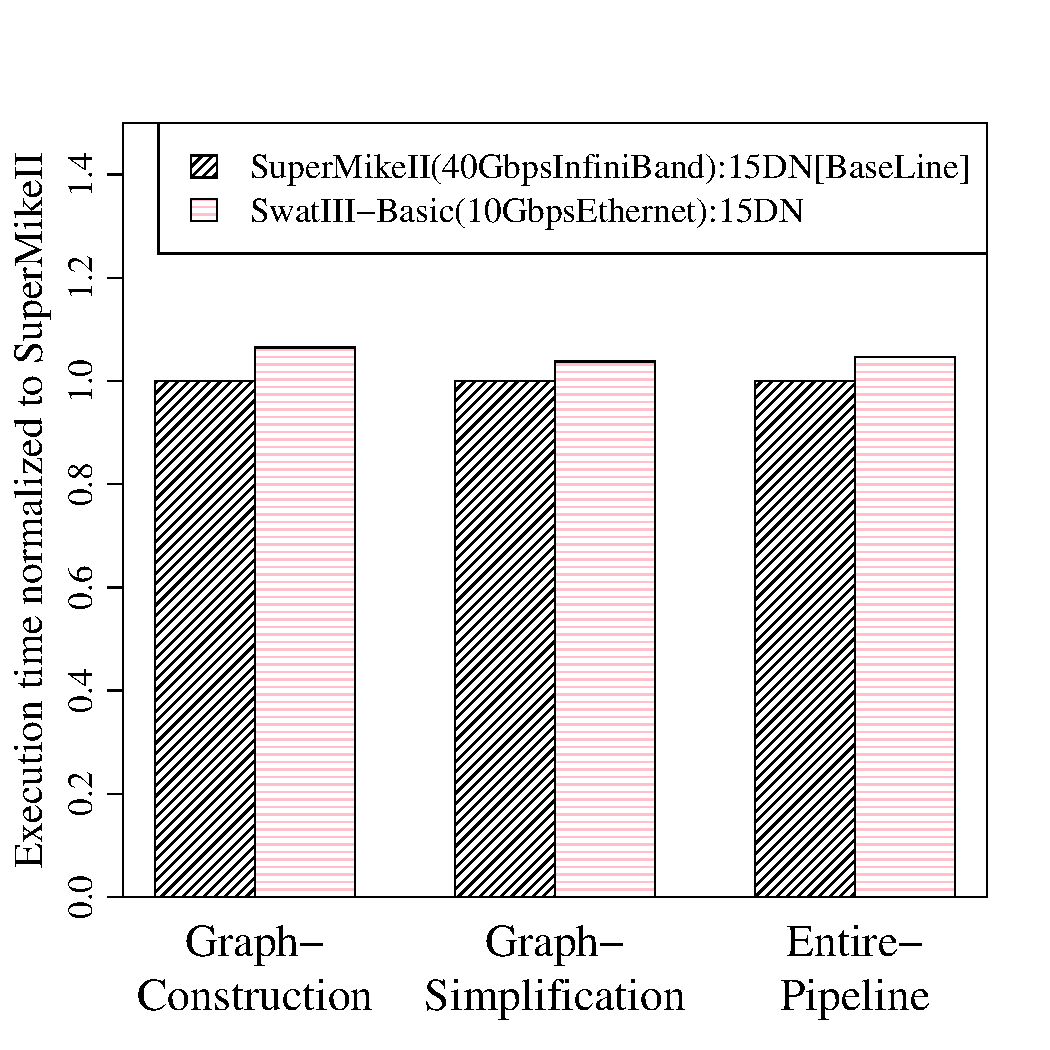
\includegraphics[width=\textwidth]{Figure/PerormanceData/Plots/Network.pdf}
                \caption{Effect of network (InfiniBand vs Ethernet).}
                \label{fig:SuperMikeSwatBasic}
        \end{subfigure}
 	\begin{subfigure}[b]{0.23\textwidth}
                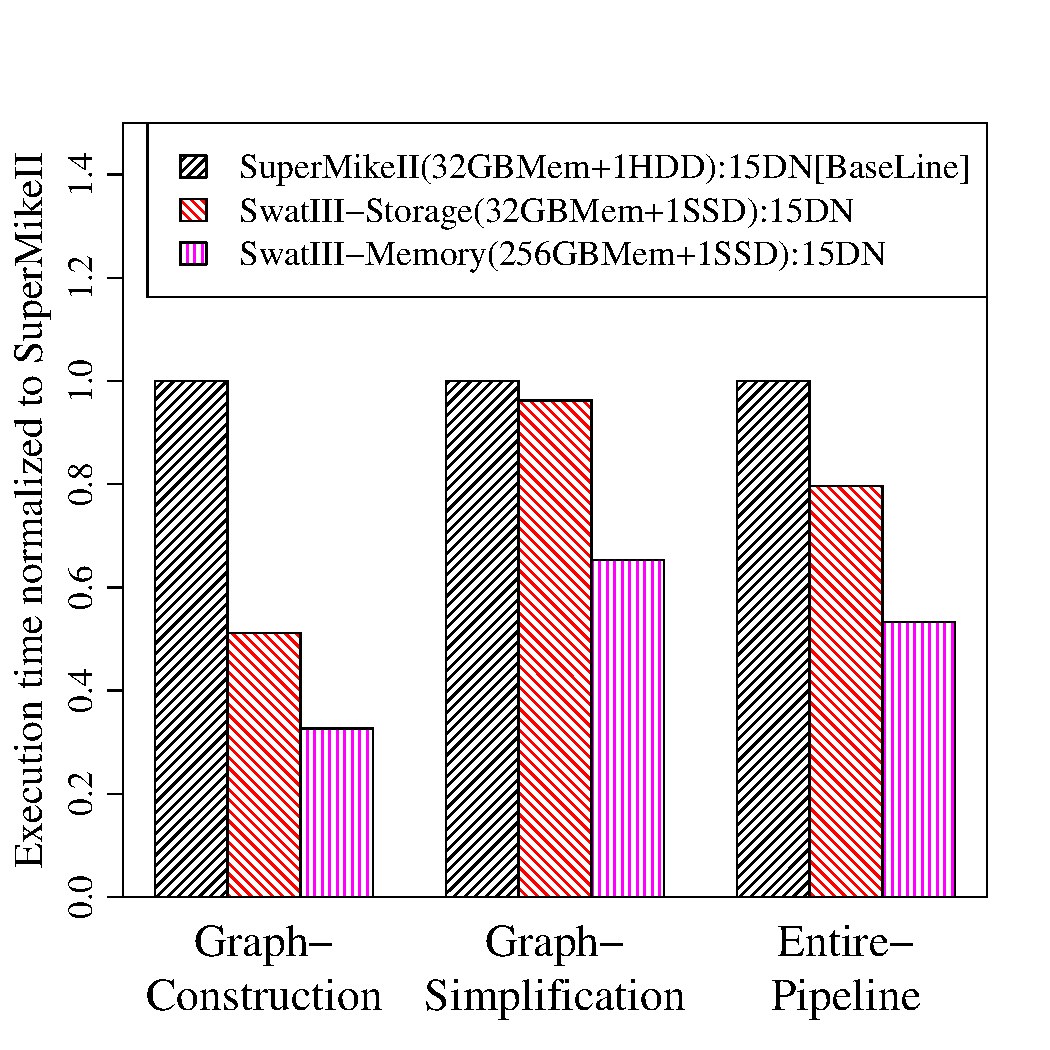
\includegraphics[width=\textwidth]{Figure/PerormanceData/Plots/StorageMemory.pdf}
                \caption{Effect of local storage (HDD vs SSD) and size of DRAM.}
                \label{fig:SuperMikeSwatStorageMemory}
   \end{subfigure}
   \caption{Impact of each individual hardware component on execution time of the assembly pipeline in 15-DN }
  \label{fig:SuperMikeSwat}
  \vspace{-1.1em}
\end{figure}
\begin{figure*}[htb]
%\centering
        \begin{subfigure}[b]{0.23\textwidth}
                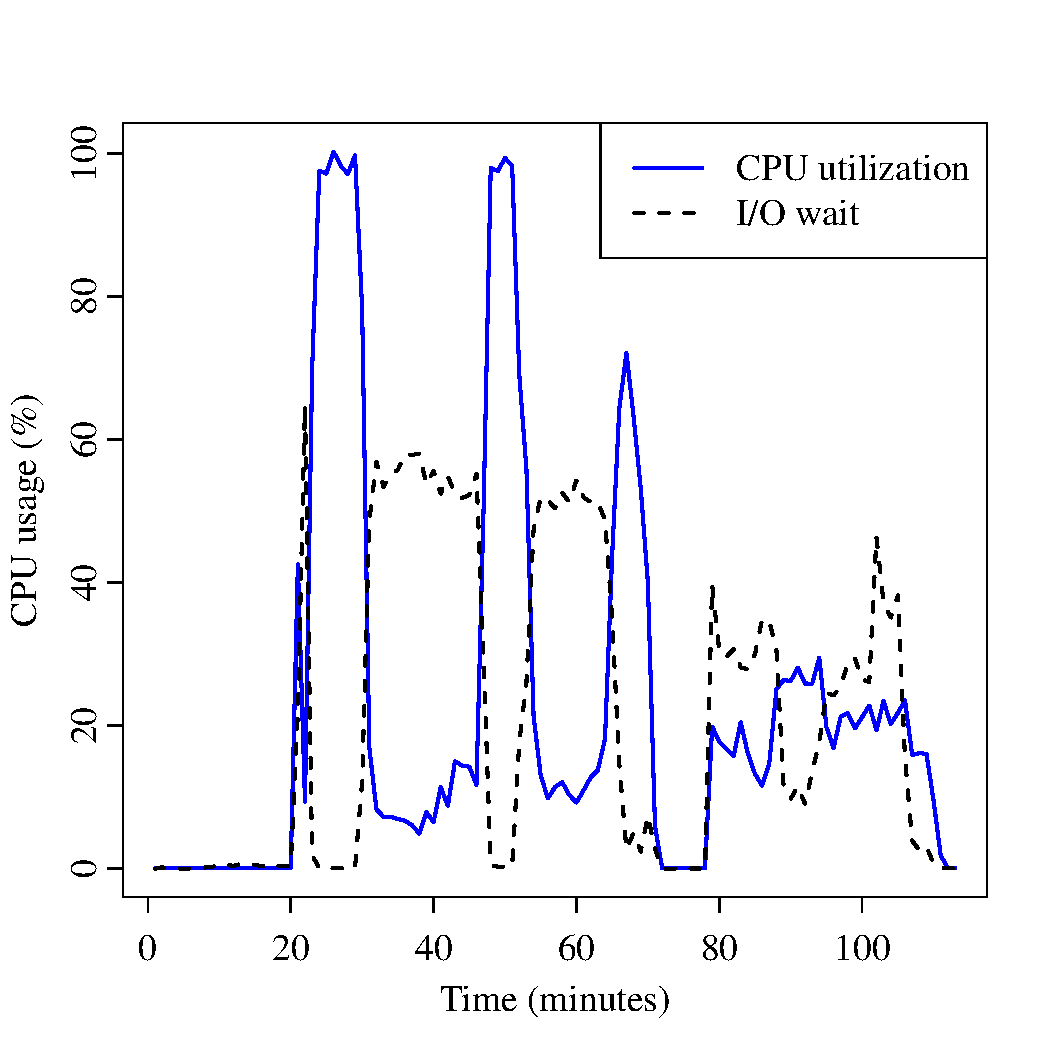
\includegraphics[width=\textwidth]{Figure/SystemData/Plots/BGCPUHDD.pdf}
                \caption{Hadoop-based graph-construction in SwatIII-Basic-HDD (1-HDD/node)}
                \label{fig:BGCPUHDD}
        \end{subfigure}
		\begin{subfigure}[b]{0.23\textwidth}
                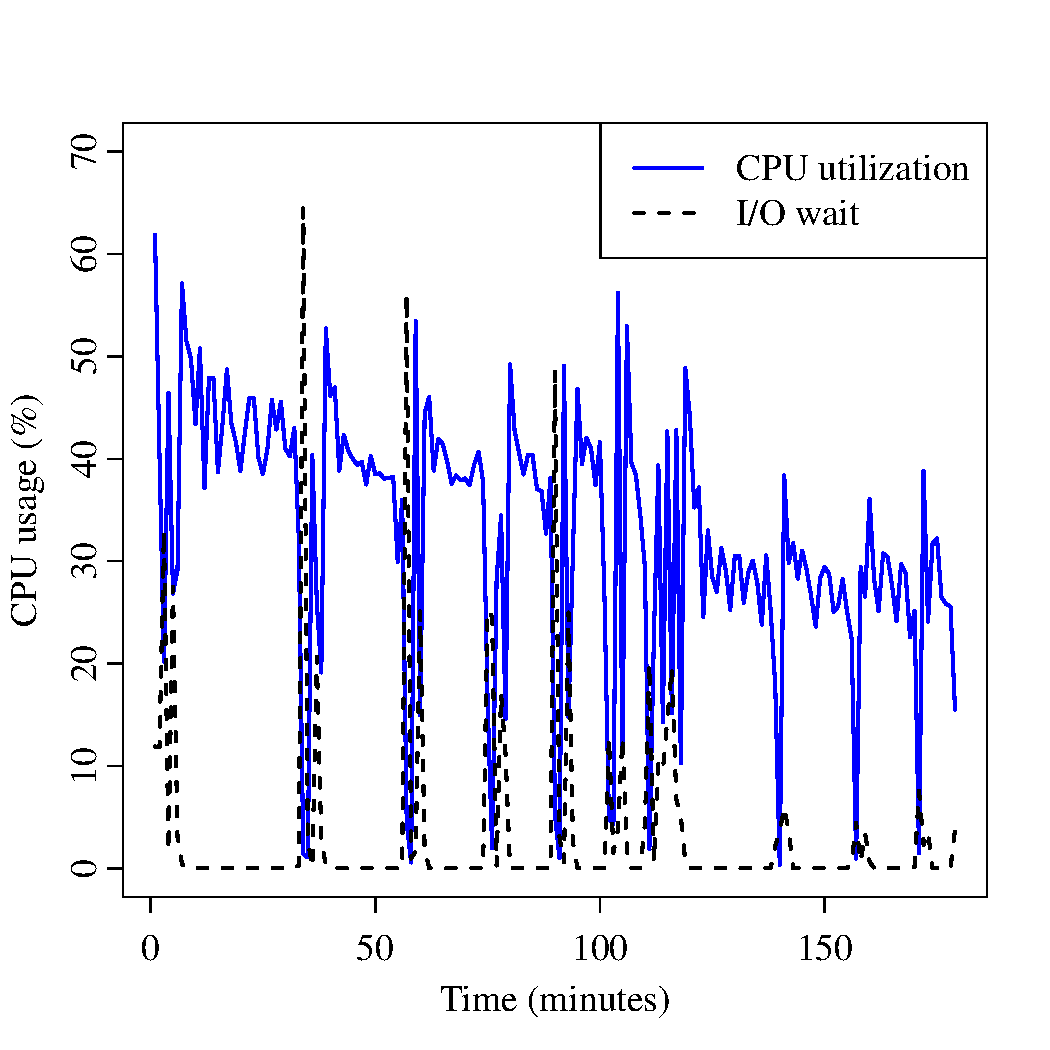
\includegraphics[width=\textwidth]{Figure/SystemData/Plots/ECCPUHDD.pdf}
                \caption{Giraph-based graph-simplification in SwatIII-Basic-HDD (1-HDD/node)}
                \label{fig:ECCPUHDD}
        \end{subfigure}       
        \begin{subfigure}[b]{0.23\textwidth}
                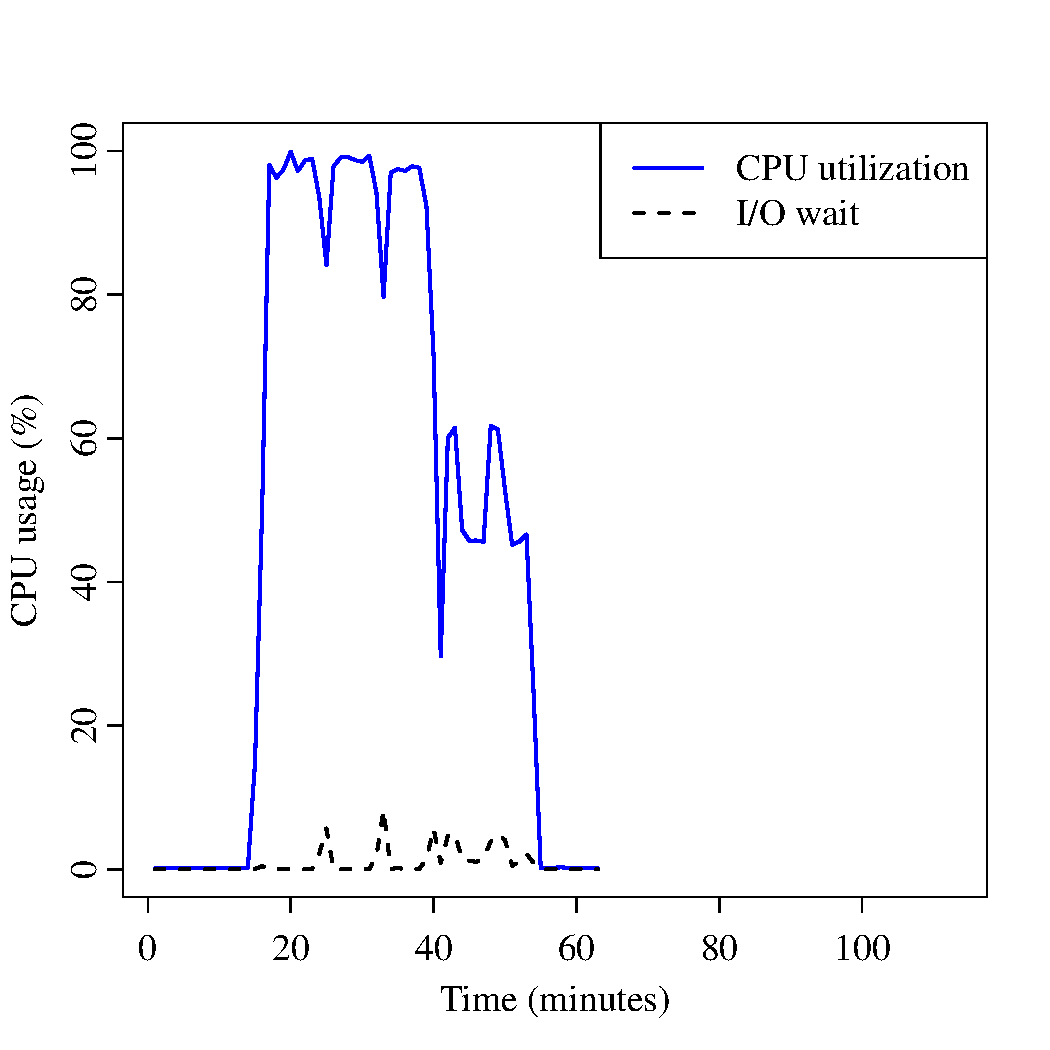
\includegraphics[width=\textwidth]{Figure/SystemData/Plots/BGCPUSSD.pdf}
                \caption{Hadoop-based graph-construction in SwatIII-Basic-SSD (1-SSD/node)}
                \label{fig:BGCPUSSD}
        \end{subfigure}    
        \begin{subfigure}[b]{0.23\textwidth}
                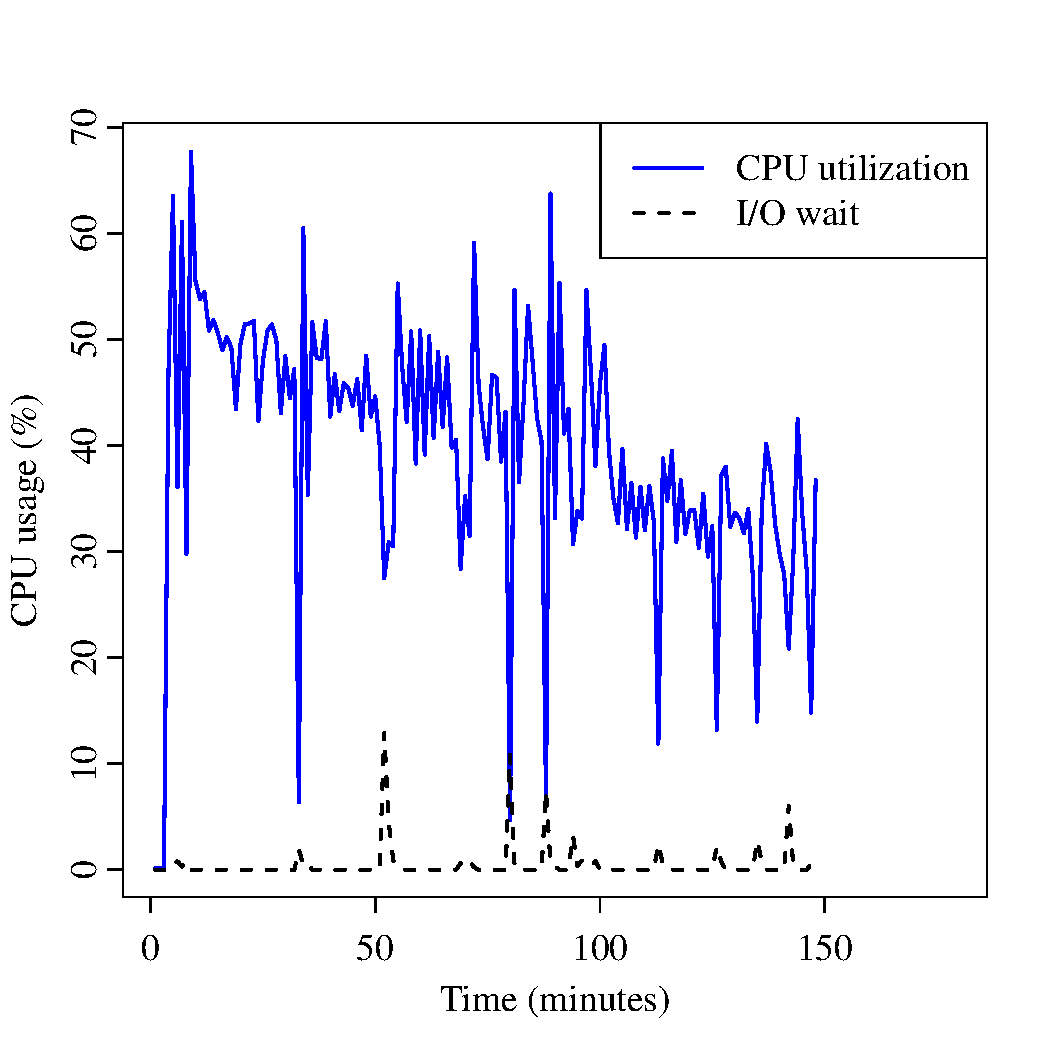
\includegraphics[width=\textwidth]{Figure/SystemData/Plots/ECCPUSSD.pdf}
                \caption{Giraph-based graph-simplification in SwatIII-Basic-SSD (1-SSD/node)}
                \label{fig:ECCPUSSD}
        \end{subfigure}
        \caption{CPU-Utilization and I/O Wait characteristics in SwatIII-Basic-HDD and SwatIII-Basic-SSD}\label{fig:HddSsdCPU}
        \vspace{-1.5em}
\end{figure*}

\begin{figure*}[htb]   
        \begin{subfigure}[b]{0.23\textwidth}
                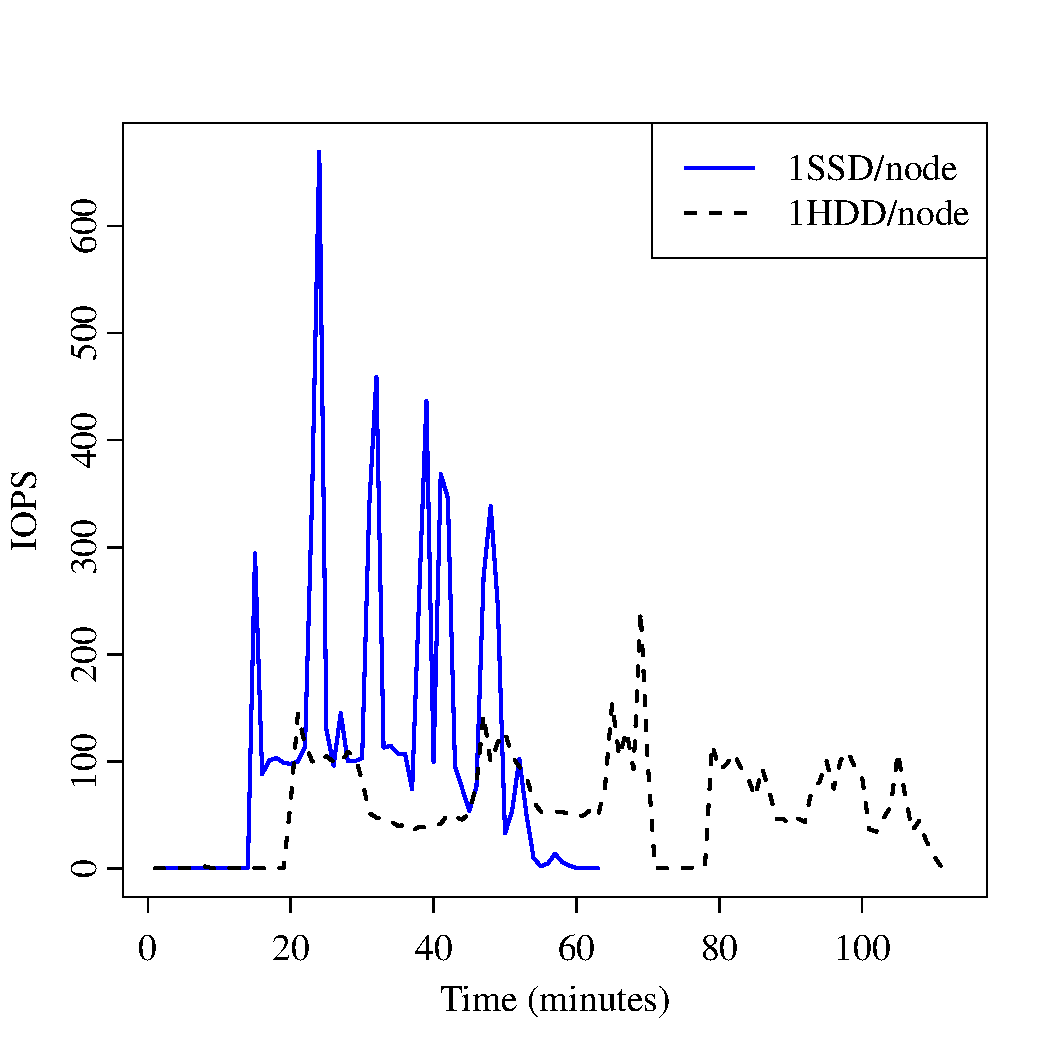
\includegraphics[width=\textwidth]{Figure/SystemData/Plots/BGHddSsdWrIops.pdf}
                \caption{Write-IOPS/DN in graph-construction in SwatIII-Basic-HDD and -SSD}
                \label{fig:BGHddSsdWrIops}
        \end{subfigure}
        \begin{subfigure}[b]{0.23\textwidth}
                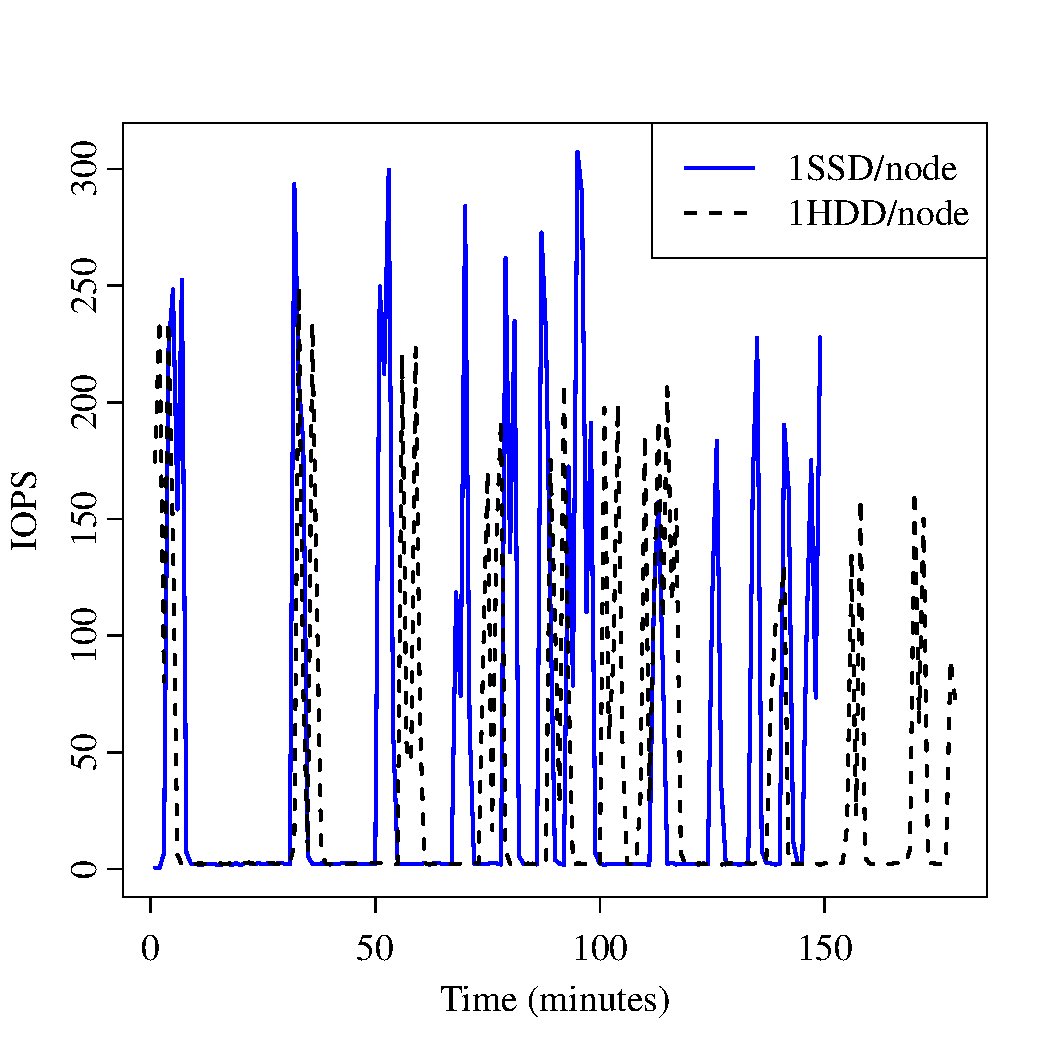
\includegraphics[width=\textwidth]{Figure/SystemData/Plots/ECHddSsdWrIops.pdf}
                \caption{Write-IOPS/DN in graph-simplification in SwatIII-Basic-HDD and -SSD}
                \label{fig:ECHddSsdWrIops}
        \end{subfigure}
        \begin{subfigure}[b]{0.23\textwidth}
                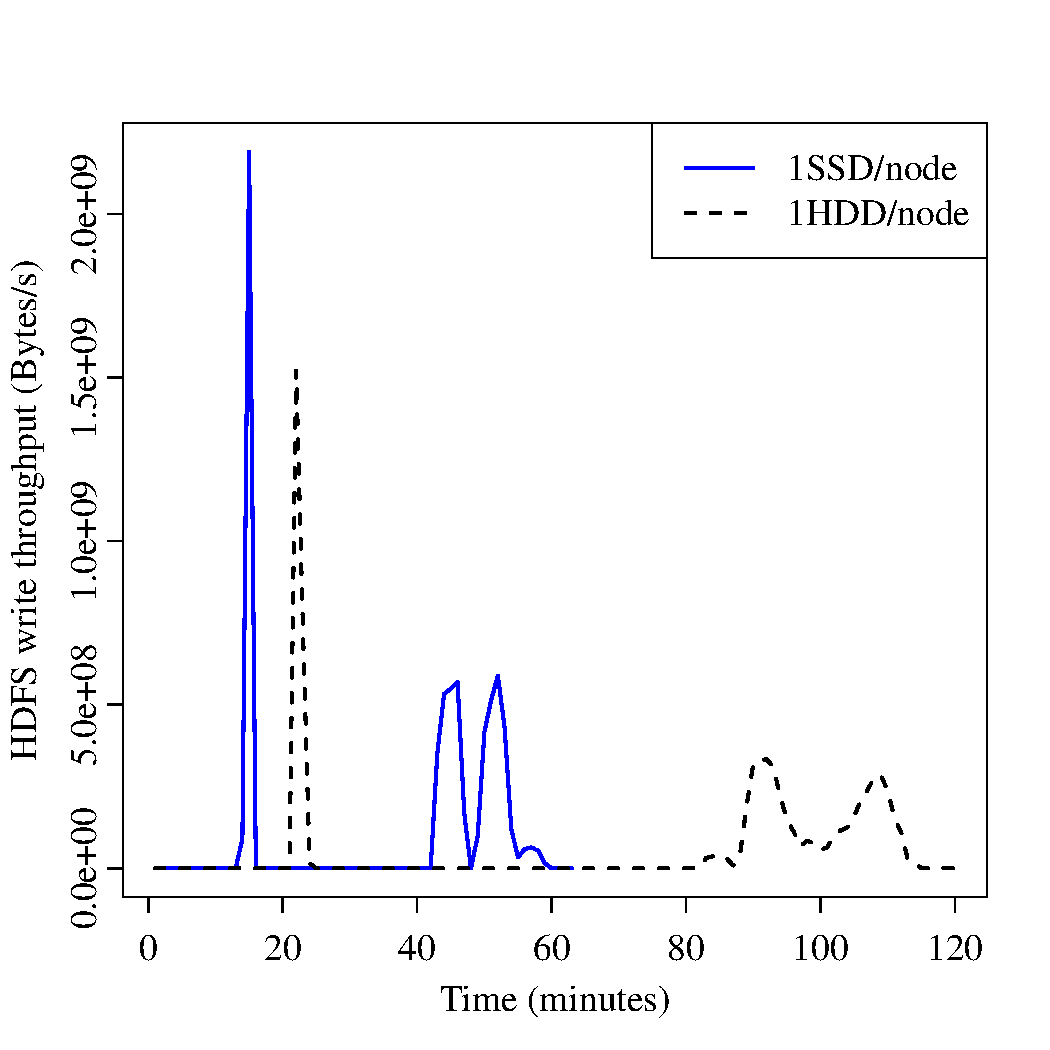
\includegraphics[width=\textwidth]{Figure/SystemData/Plots/BGHddSsdHdfsWrIops.pdf}
                \caption{HDFS-Write-throughput in graph-construction in SwatIII-Basic-HDD and -SSD}
                \label{fig:BGHddSsdHdfsWrIops}
        \end{subfigure}
        \begin{subfigure}[b]{0.23\textwidth}
                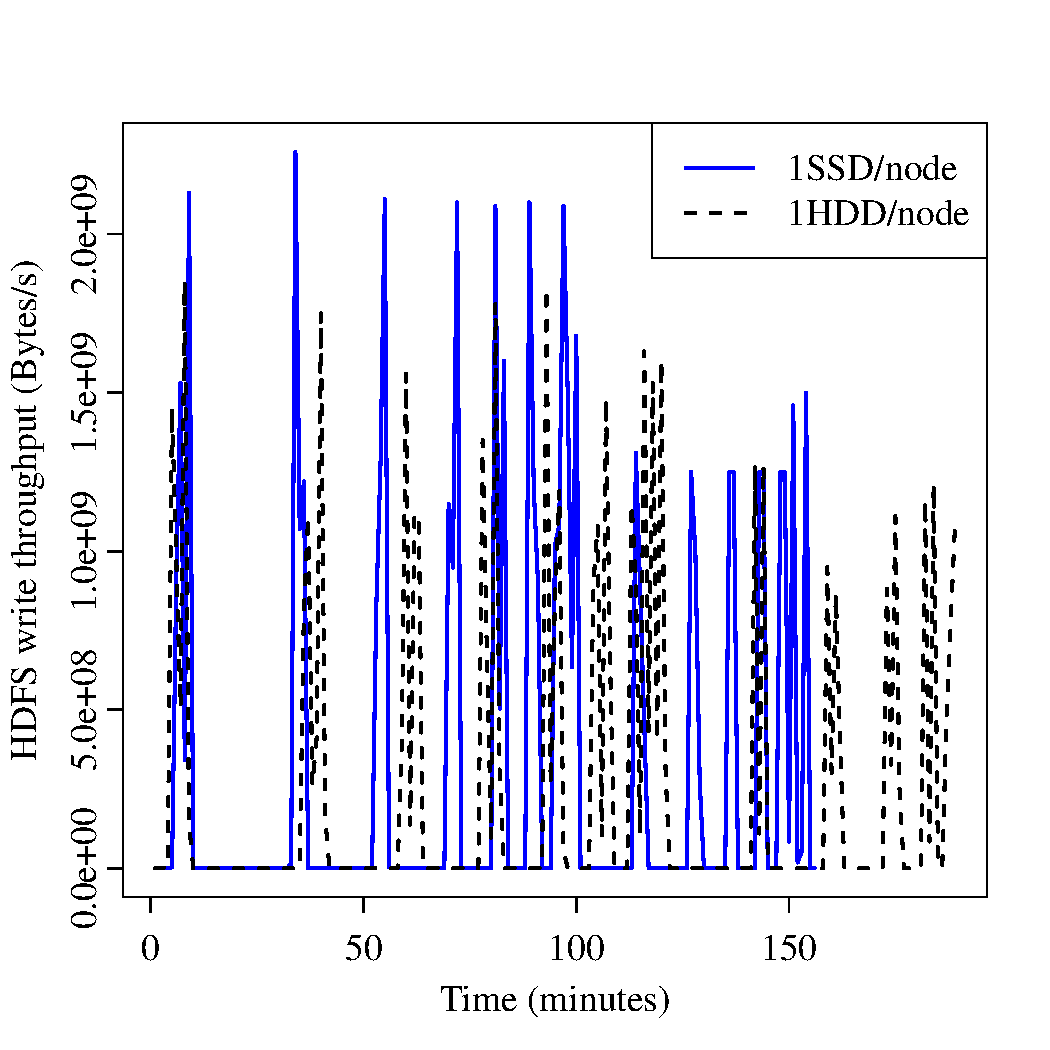
\includegraphics[width=\textwidth]{Figure/SystemData/Plots/ECHddSsdHdfsWrIops.pdf}
                \caption{HDFS-Write-throughput in graph-simplification in SwatIII-Basic-HDD and -SSD}
                \label{fig:ECHddSsdHdfsWrIops}
        \end{subfigure}       
        \caption{Comparison of IOPS (write) on Local File System (of each datanode) and I/O throughput for HDFS-write (across all DNs) for HDD and SSD. The shuffle phase of Hadoop gains maximum from SSD.}\label{fig:HddSsdHdfsRWps}   
        \vspace{-1.5em}
\end{figure*}
\begin{figure*}[htb]
        \begin{subfigure}[b]{0.5\textwidth}
                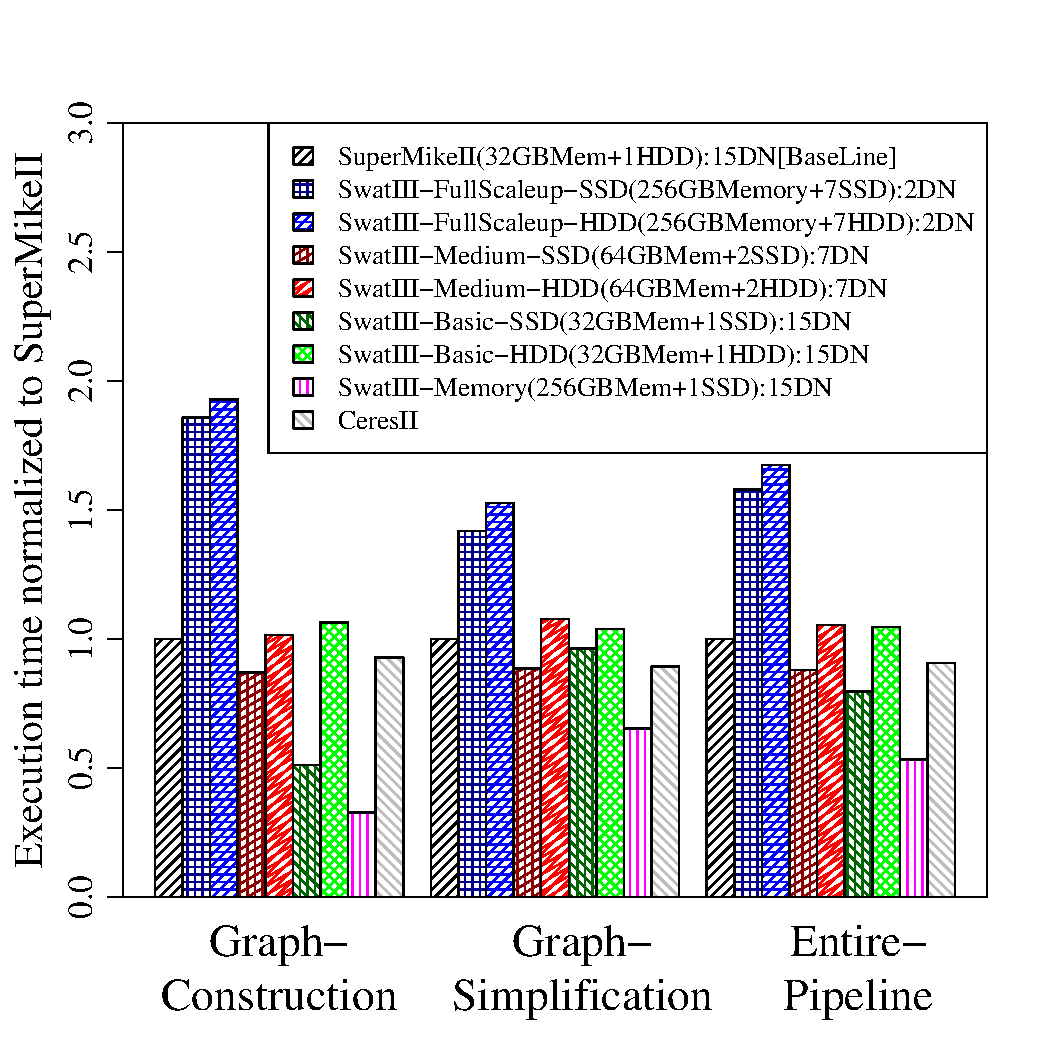
\includegraphics[width=\textwidth, height=.27\textheight]{Figure/PerormanceData/Plots/PerfDiffArch.pdf}
                \caption{Execution time (Lower execution time means better performance)}
                \label{fig:DifferentArchitecturesPerf}
        \end{subfigure}
        \begin{subfigure}[b]{0.5\textwidth}
                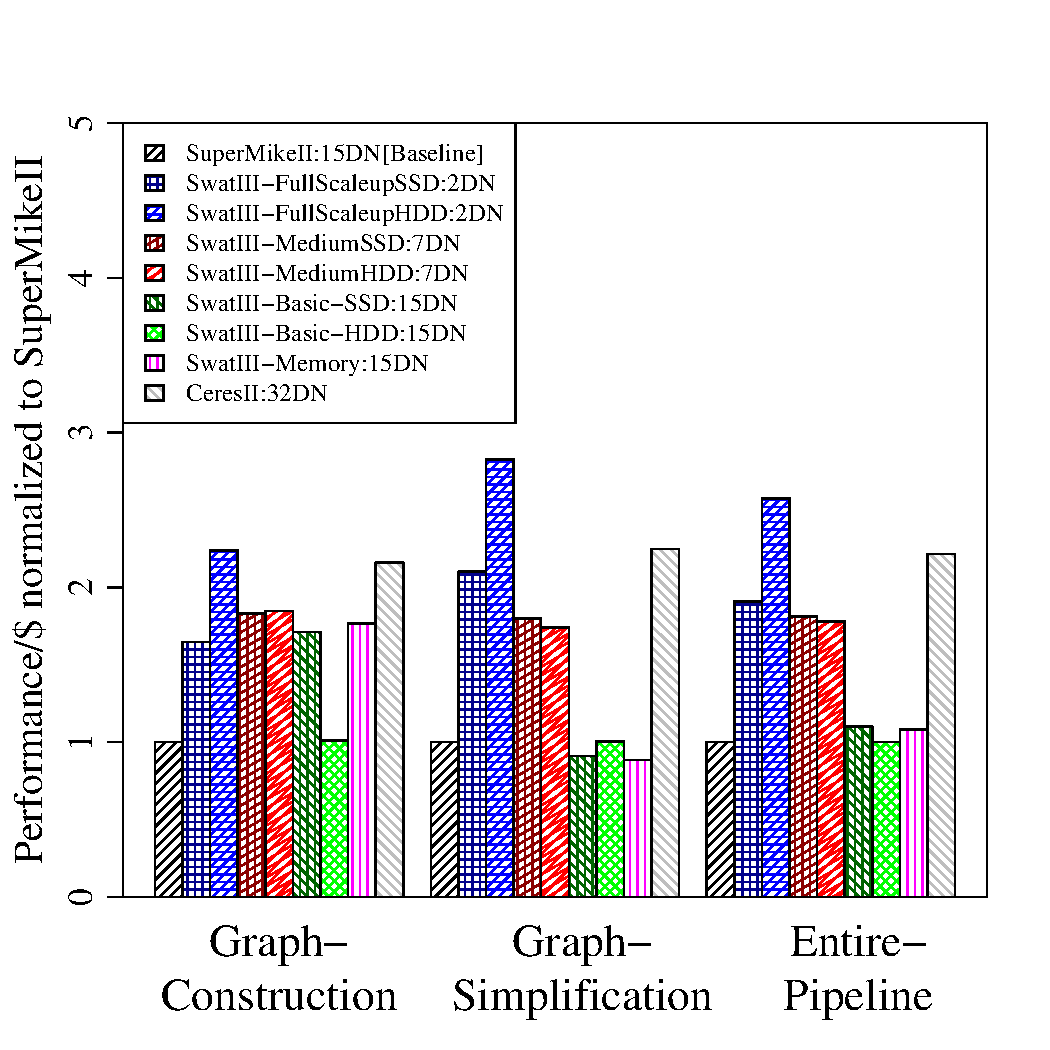
\includegraphics[width=\textwidth, height=.27\textheight]{Figure/PerormanceData/Plots/PerfPerDollarDiffArch.pdf}
                \caption{Performance-to-Price (Higher performance per dollar is better)}
                \label{fig:DifferentArchitecturesPerfPerDollar}
        \end{subfigure}
        \caption{Comparison among different type of cluster architectures in terms of execution time and performance-to-price}
  \label{fig:DifferentArchitectures}
  \vspace{-1em}
\end{figure*}
In this section, we compare the individual impact of each hardware component, such as, network, storage, and memory individually on our benchmark genome assembler. To do that, we use 16 nodes in both SuperMikeII and SwatIII. Each node in both the clusters has 16 processing cores. We started with comparing the impact of the network between SuperMikeII and SwatIII-Basic-HDD. Then, we further optimized those 16 nodes of SwatIII cluster incrementally in terms of storage by providing SSD (named as SwatIII-Basic-SSD) and then providing more memory to each node (named as SwatIII-Memory). The execution-times reported in this section are the means of at least 3 runs of the assembler on each different hardware configuration.
\label{IndividualHWEffect}

\subsection {Effect of Network: InfiniBand vs Ethernet} \label{EffectOfNetwork}
Figure-\ref{fig:SuperMikeSwatBasic} compares the impact of network interconnect on PGA while assembling a 90GB bumble bee genome. The execution time is normalized to the SuperMikeII-baseline. We did not find any visible performance difference (less than 2\%) on any of the stages of our assembly pipeline even though SuperMikeII uses 40-Gbps QDR InfiniBand and SwatIII-Basic-HDD uses a 10-Gbps Ethernet. The reason is as follows: although the average latency in SuperMikeII is almost $1/14$ of that in SwatIII ($0.014$ms in SuperMikeII compare to $0.2$ms in SwatIII), the average effective bandwidth between any two SuperMikeII nodes is 10-times lower than that of SwatIII ($954$Mbit/s in SuperMikeII, whereas $9.2$Gbit/s in SwatIII) because of the $2:1$ blocking ratio in the InfiniBand network.  

\subsection {Effect of local storage device: HDD vs SSD} \label{EffectOfSSD}
Figure-\ref{fig:SuperMikeSwatStorageMemory} compares the execution time of SwatIII-Basic-SSD to the SuperMikeII-baseline. The second column of each stage of the assembler in Figure-\ref{fig:SuperMikeSwatStorageMemory} shows the impact of using SSD in that stage of the assembly. We observed almost 50\% improvement in the shuffle intensive graph-construction stage because of reduced I/O wait. However, graph-simplification, a series of in-memory Giraph jobs (that read/write data only to the HDFS), is not affected much (less than 3\%) by using SSD. 
 
Actually, the shuffle phase of Hadoop experiences maximum I/O wait when a many I/O threads work concurrently to spill and subsequently read huge data to/from the disk. This I/O wait is significantly reduced using SSD (Figure-\ref{fig:BGCPUSSD} and -\ref{fig:ECCPUSSD}) resulting in remarkable performance improvement in Hadoop. However, for Giraph we did not observe any notable improvement using SSD because of very less I/O wait. Basically, an SSD increases the disk IOPS per DataNode by 7 to 8 times than an HDD improving the shuffle phase's CPU utilization as shown in Figure-\ref{fig:BGHddSsdWrIops}. In case of Giraph, the corresponding improvement is 1.5-times as shown in Figure-\ref{fig:ECHddSsdWrIops}. Considering the I/O throughput to HDFS, we also observed 1.5-times improvement in case of SSD for both Hadoop and Giraph as shown in Figure-\ref{fig:BGHddSsdHdfsWrIops} and -\ref{fig:ECHddSsdHdfsWrIops}. Giraph, which writes data to the HDFS only, shows the similar I/O characteristics  for both IOPS per DataNode (DN) and HDFS I/O throughput because they are related by the equation: $HDFS\_IO\_Throughput = IOPS\_per\_DN \times Bytes\_per\_IO \times \#DN$, where $Bytes\_per\_IO$ is the characteristics of the disk. However, for Hadoop, these characteristics are different as it writes lots of data to local file system during shuffle phase.

\subsection {Effect of size of DRAM} \label{EffectOfDRAM}
The third columns of Figure-\ref{fig:SuperMikeSwatStorageMemory} shows the impact of increasing the amount of memory per node. We observed almost 20\% improvement in the initial graph-construction phase from SwatIII-Basic-SSD, i.e., almost 70\% improvement to the baseline. In the Giraph phase, the corresponding improvement is 35\%. The improvement is mostly because of the caching. Especially, in case of Giraph, where computation proceeds in iterative supersteps, a huge amount of data is cached and is fetched upon requirement during the next compute-superstep.

\section {Impact of Different Hardware Organization} \label{ComparingDifferentArchitecturalBalance}

In this section, we compare different cluster architecture in terms of execution time and performance-to-price. Again, the execution-times are the means of at least 3 runs of the assembler on each different hardware configuration.

\subsection {Execution time comparison between SuperMikeII and SwatIII variants (with moderate-size bumble bee genome)} \label{ExecutionTimeDiffArchBumblebee}
Figure-\ref{fig:DifferentArchitecturesPerf} shows the relative merits of different cluster architectures in terms of raw execution time. Observe that we always keep the total aggregated storage and memory space almost same across all the clusters (Except the SwatIII-Memory). The basic assumption behind this experimental setup is that the total amount of data should be held in its entirety in any of the cluster. The observations are as follows:
\begin{inparaenum}[\itshape 1\upshape)]
\item \textbf{SwatIII-Basic (16-DNs):} As discussed earlier in Section-\ref{IndividualImpactofDifferentHardwareConfiguration}, for Hadoop, the SSD variant of this scaled out cluster shows $2$x speedup over the baseline whereas the HDD variant performs similar to the baseline. For Giraph, both of them perform similar to the baseline.
\item \textbf{SwatIII-FullScaleup (2-DNs):} This scaled up small sized cluster takes the maximum time for any workload because of least number of processing cores. Observe that for the Hadoop job, both SSD and HDD variants of this scaled up configuration perform similarly, which is in contrast with scaled out SwatIII-Basic. We discuss it in more detail in Section-\ref{ScaledupClusterAndSSD}.
\item \textbf{SwatIII-Medium (7-DNs):} The HDD variant of this cluster perform similar to the baseline for both Hadoop and Giraph even though the total number of cores in the cluster is half of the baseline. It is because 2-HDDs and 64GB RAM per node increase the IOPS and the caching respectively. The SSD variant shows slightly better result than the HDD because of further increase in IOPS.
\item \textbf{SwatIII-Memory (16-DNs):} It is no surprise that this configuration shows the lowest execution time among all because of the maximum resource availability.
\end{inparaenum}

\subsection {Performance-to-Price comparison between SuperMikeII and SwatIII variants (with the bumble bee genome)} \label{PriceToPerformanceBumbleBee}
We consider the performance as the inverse of the execution time and divided it by the total cost of the cluster to get the performance/\$. Because of similar total memory and storage space across clusters none of them gets price benefit over other in terms of storage and memory. Rather, we compare the performance to price from the view point of a proper architectural balance among number of cores, number of disks, and amount of memory per node. We did not consider the cost of network for a fair comparison with SuperMikeII, the public HPC cluster that is shared among many users.

Figure-\ref{fig:DifferentArchitecturesPerfPerDollar} compares the performance/\$ metric among all the clusters. The observations are as follows:
\begin{inparaenum}[\itshape 1\upshape)]
\item \textbf{SwatIII-Basic:} For Hadoop, the SSD variant of this scaled out cluster shows 2-times better performance/\$ comparing to the baseline as well as to its HDD variant. However, for Giraph, it does not add any benifit.
\item \textbf{SwatIII-FullScaleup:} Although this small scaled up cluster takes shows maximum execution time, it shows high performance/\$ for both Hadoop and Giraph. For Hadoop, the SSD and HDD variants show 1.5 and 2.5 times benefit to the baseline respectively. For Giraph, the corresponding benefit is 2 and 3 times respectively for SSD and HDD.The HDD variant obviously shows better performance/\$ than the SSD as their execution time is similar. This is again in contrast with the scaled out (SwatIII-Basic) case.
\item \textbf{SwatIII-Medium:} Both the HDD and SSD variant of this configuration shows similar result, almost 2-times better than the baseline for both Hadoop and Giraph. Considering both performance and the price, it is the most optimal configuration in our evaluation.
\item \textbf{SwatIII-Memory}: For Hadoop, it shows 2-times benefit to the baseline. However, once SSD is used as the underlying storage more memory do not add any advantage in terms of performance/\$ (comparing to SwatIII-Basic-SSD). For Giraph, it does not have any impact on performance/\$ comparing to the baseline. 
\end{inparaenum}

\subsection {Comparing SuperMikeII and SwatIII (with large human-genome)} \label{SecPerfDiffArchHum}
\vspace{-1.9em}
\begin{figure}[htb]
\center
        \begin{subfigure}[b]{0.23\textwidth}
                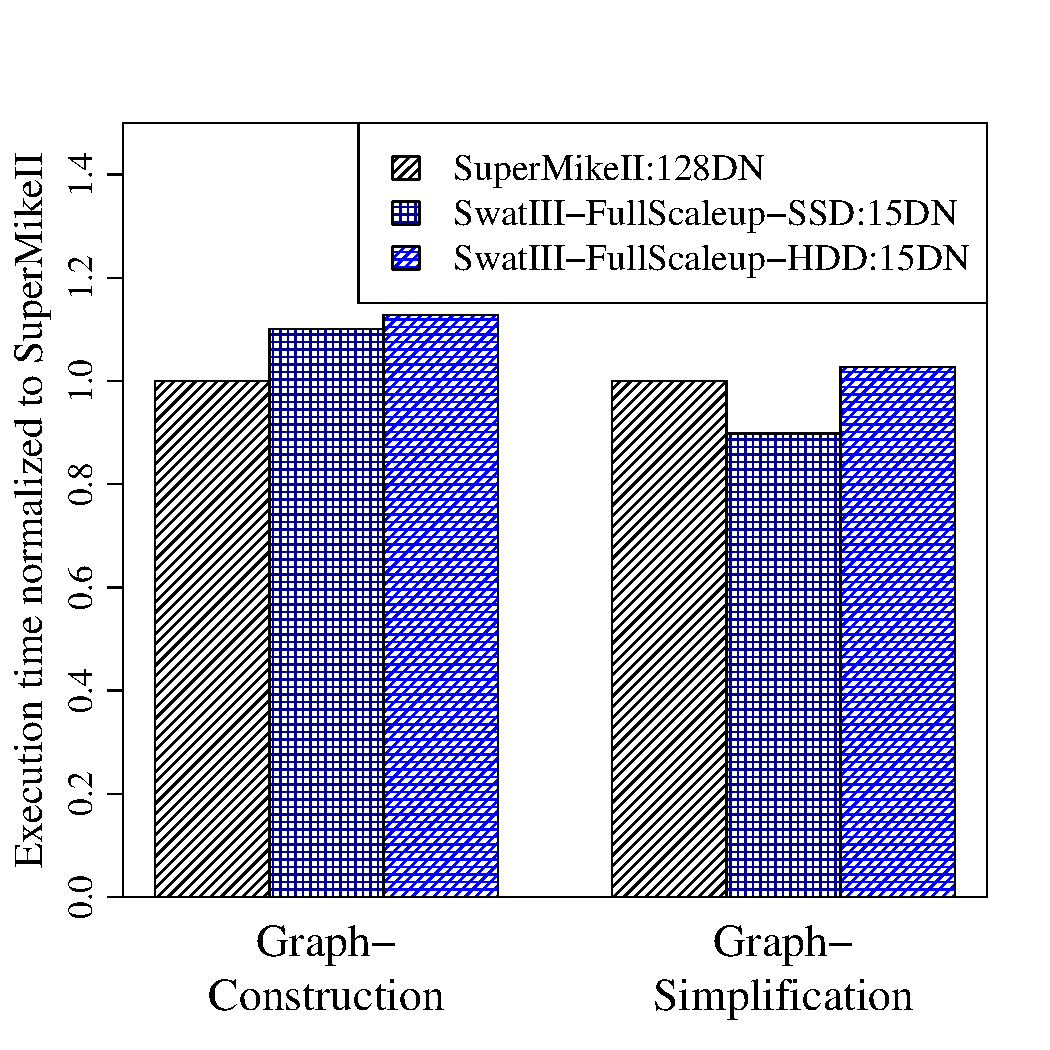
\includegraphics[width=\textwidth]{Figure/PerormanceData/Plots/PerfDiffArchHum.pdf}
                \caption{Execution time (Lower execution time is better).}
                \label{fig:DifferentArchitecturesPerfHum}
        \end{subfigure}
        \begin{subfigure}[b]{0.23\textwidth}
                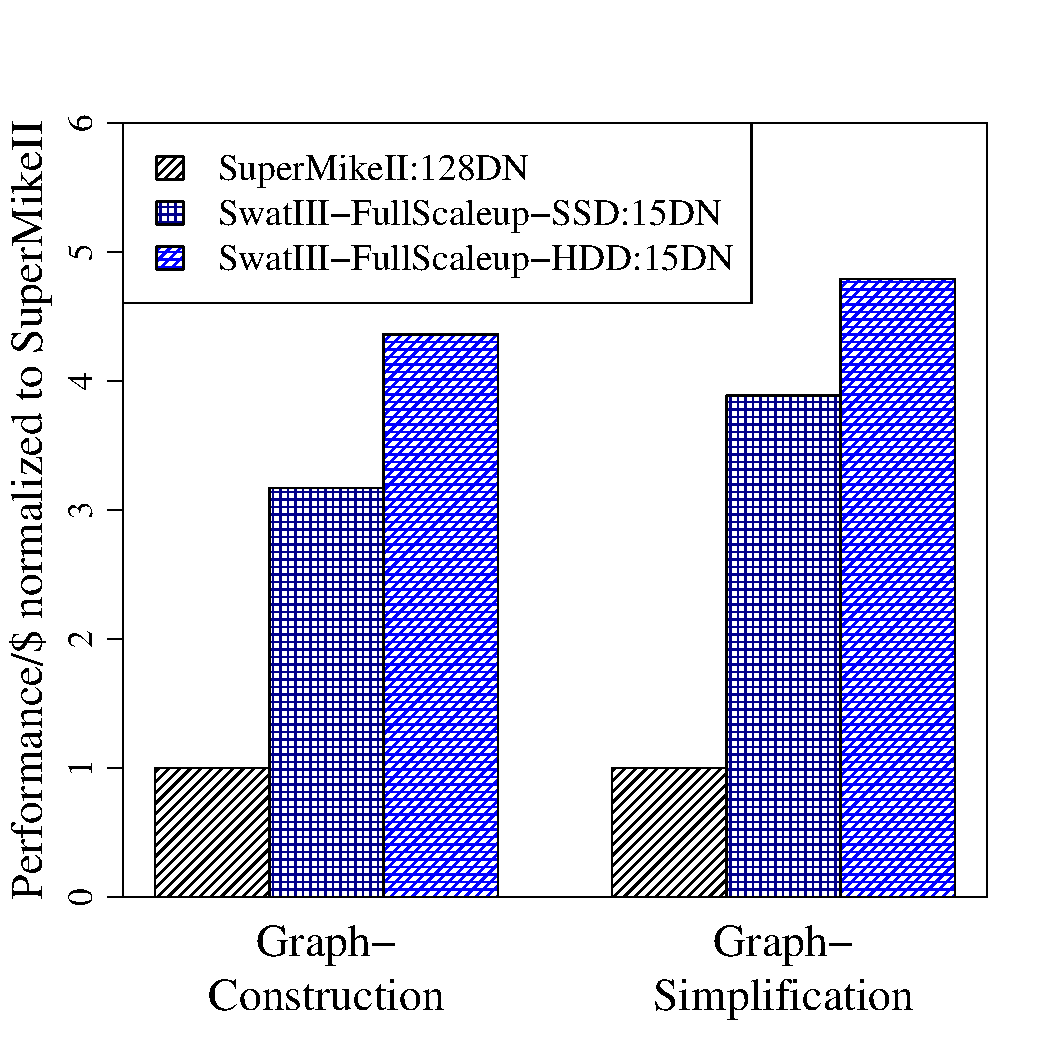
\includegraphics[width=\textwidth]{Figure/PerormanceData/Plots/PerfPerDollarDiffArchHum.pdf}
                \caption{Performance/\$ (Higher performance/\$ is better).}
                \label{fig:DifferentArchitecturesPerfPerDollarHum}
        \end{subfigure}
        \caption{Comparison of different types of cluster architecture for human genome assembly pipeline.}
  \label{fig:DifferentArchitecturesHum}
  \vspace{-.8em}
\end{figure}
The large human genome (452GB)  produces huge amount of shuffled data (9.9TB) as well as the graph data (3.2TB). We use 127 DataNodes in SuperMikeII and 15 DataNodes in the SwatIII-Full-Scaleup for this. Figure-\ref{fig:DifferentArchitecturesPerfHum} and \ref{fig:DifferentArchitecturesPerfPerDollarHum} shows the execution time and the performance/\$ respectively for the human genome assembly pipeline. The observations are as follows:
\begin{inparaenum}[\itshape 1\upshape)]
\item For Hadoop, the 127-DNs of SuperMikeII (2032-cores) show only 15-17\% better performance than 15-DNs (240 cores) of SwatIII-FullScaleup cluster (any variant) while using 8.5-times more cores. The reasons behind the lower performance in SuperMikeII are both the huge I/O and network bottleneck as discussed earlier in Section-\ref{Bigdata Softwares on Traditional Supercomputers}. Again, observe that for this large data set also, both SwatIII-FullScaleup-HDD and SSD perform similarly.
\item For the Giraph-based graph-simplification stage also, SuperMikeII did not show the expected performance mainly because of the low network bandwidth resulted by 2:1 blocking.  
\item In terms of performance/\$ the scaled up configuration shows huge gain over the baseline. For Hadoop, the gain is 3 to 5 times based upon the storage media. For Giraph, the corresponding gain is almost 4 to 5 times. Again, because of the similar execution time, the scaled up HDD variant shows better performance/\$ than the SSD variant.
\end{inparaenum}

\subsection {Performance of SSD in scaled out and scaled up cluster} \label{ScaledupClusterAndSSD}
\vspace{-1.9em}
\begin{figure}[h]
  \centering
  \begin{subfigure}[b]{0.23\textwidth}
          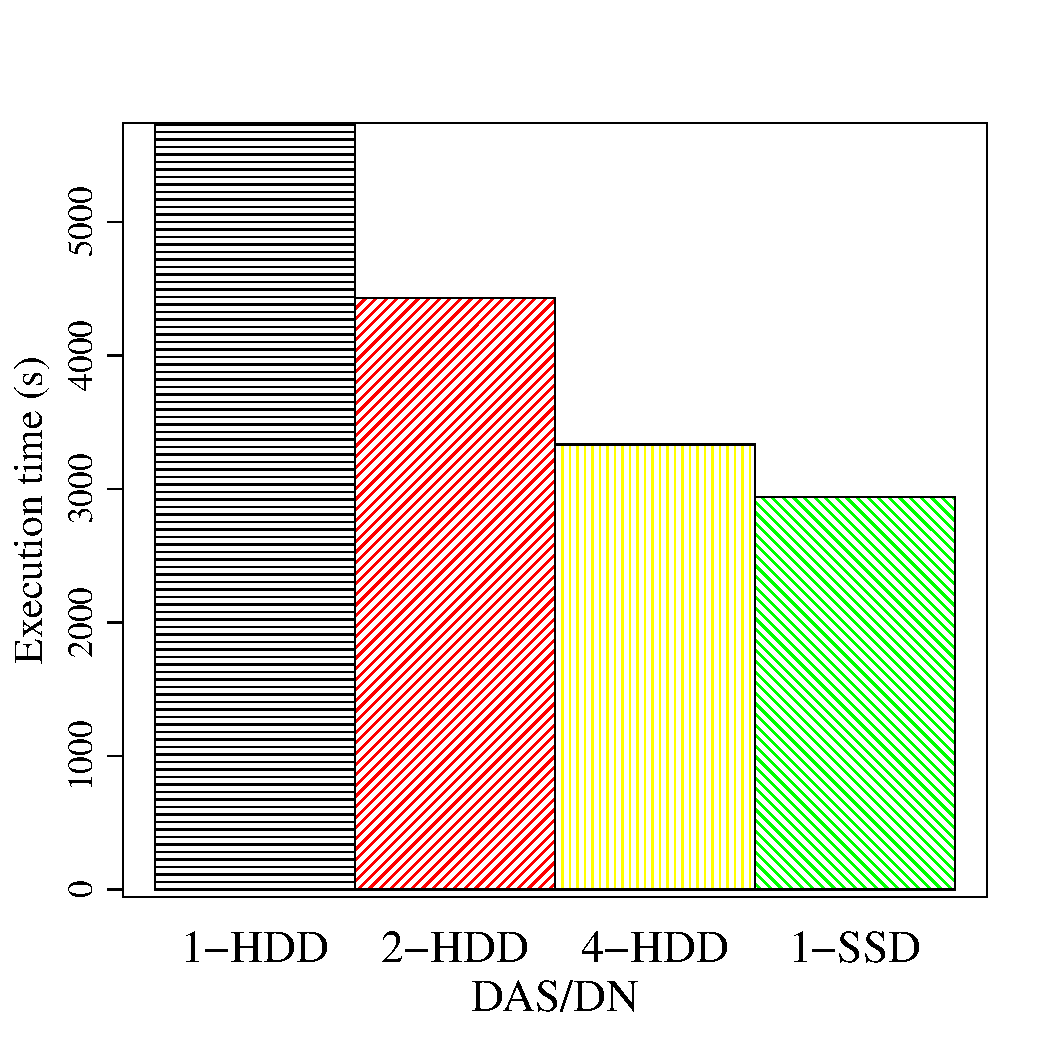
\includegraphics[width=\textwidth]{Figure/PerormanceData/Plots/SSDHDDSameNode.pdf}
          \caption{Hadoop performance trend using 1, 2 and 4 HDD(s) and 1-SSD per node using 15 datanodes in the cluster.}
          \label{fig:SsdN4Hdd}
  \end{subfigure}
  \begin{subfigure}[b]{0.23\textwidth}
          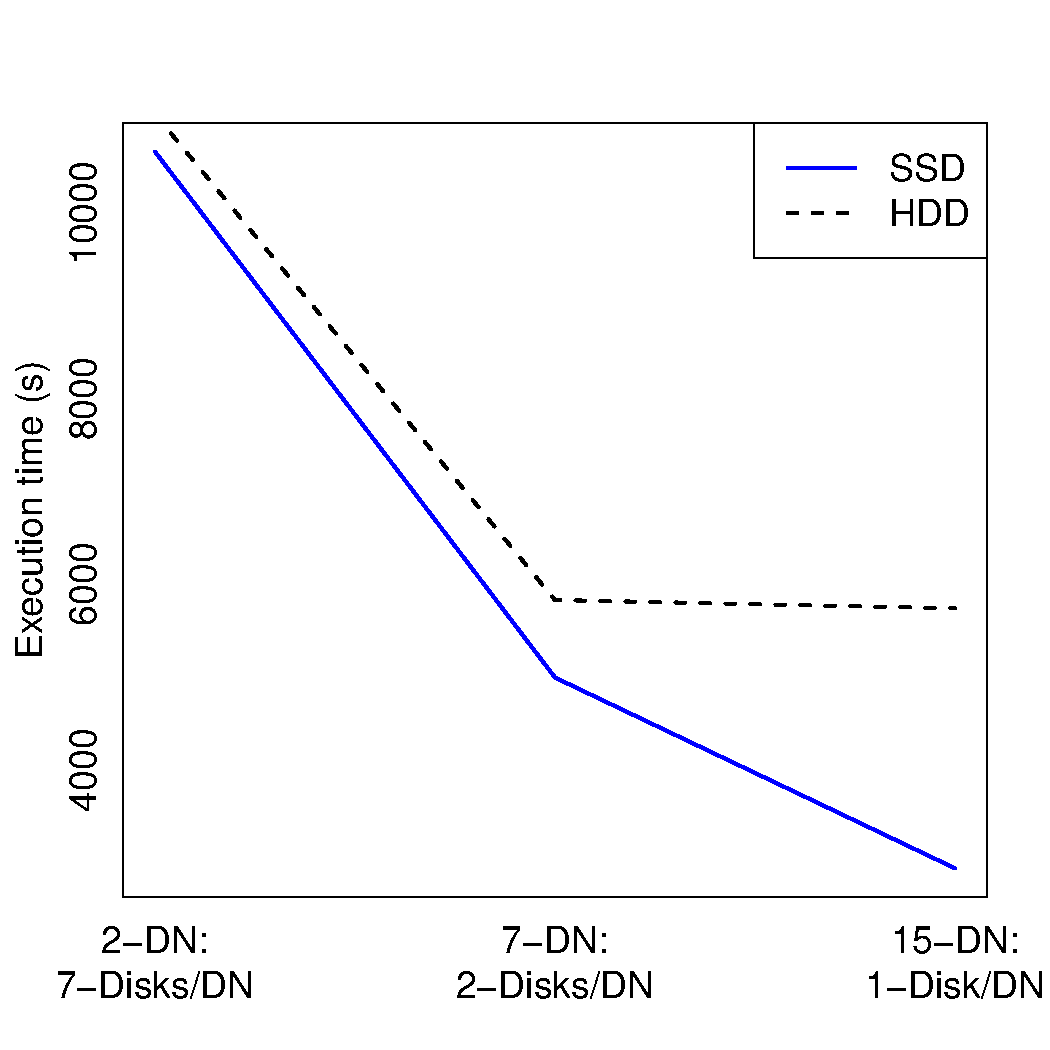
\includegraphics[width=\textwidth]{Figure/PerormanceData/Plots/SSDHDDDiffNode.pdf}
          \caption{Hadoop performance trend for SSD and HDD using 1, 2, 7 disks per node in 15, 7 and 2 datanodes in the cluster.}
          \label{fig:SsdNHddDiffNodes}
  \end{subfigure}
  \caption{Performance trend using HDD and SSD in Hadoop. SSD shows better performance and sclability in a scaled out environment}
  \label{fig:SsdNHdd}
  \vspace{-.8em}
\end{figure}
Storage optimized, scaled up cloud instances frequently come with 4 to 8-SSDs per instance to improve the performance, consequently incurring high setup-cost and service-charge. For example, AWS-i2.8xlarge offers 8-SSDs per instance at a rate of \$6.82/hour. But, is it the effective way to deploy the SSDs? The disk controllers saturate after a certain I/O throughput (an observation by Szalay \cite{cluster:AmdahlBalancedBlade}). In this section, we compare the performance characteristics of HDD and SSD in both scaled out and scaled up environment.

Figure-\ref{fig:SsdN4Hdd} compares the performance of a single SSD and increasing number of HDDs per node for the Hadoop stage of the bumble bee genome assembly using 15-DNs. The performance improves almost linearly by increasing the number of HDDs per node in the cluster. On the other hand, 4-HDDs per node shows similar performance (only 5\% variation) with a single-SSD per node. At this I/O thoughput the disk controller saturates, and adding more disk(s) to the nodes does not improve the performance. Both Figure-\ref{fig:SsdNHddDiffNodes} as well as Figure-\ref{fig:DifferentArchitecturesPerfHum} substantiate our claim for moderate-size bumble bee and large-size human genome data. For both the data, both the HDD and SSD variant of SwatIII-FullScaleup perform similarly where each DN is equipped with 7-disks. However, SSD showed significantly better performance and scalability than HDD when we scaled out by adding more compute nodes to the cluster.

\subsection {Performance of CeresII: Samsung MicroBrick with PCIe communication} \label{CeresII:Scaledout-in-a-boxAndSSD}
In this section, we evaluate a Samsung MicroBrick-based novel CeresII architecture. Currently CeresII is in prototype phase. As mentioned before, CeresII uses 2 physical cores, 1-SSD and 16GB memory per compute server and uses a PCIe-based interface to communicate among high-density compute-servers in a chassis. The PCIe based communication improves efficiency of the cluster enormously by reducing the communication overhead. At the same time, the SSD based MicroBricks enable efficient resource utilization in a significantly low cost. 

To assemble the 95GB bumble bee genome we use 32 compute-servers of CeresII as Hadoop DNs. The last columns in Figure-\ref{fig:DifferentArchitecturesPerf} and Figure-\ref{fig:DifferentArchitecturesPerfPerDollar} show the execution-time and performance/\$ respectively for CeresII for different stages of the assembly. CeresII always shows the similar execution time to the baseline while producing more than 2-times improvement in performance/\$.

From the performance comparison between SuperMikeII and SwatIII, we noticed a huge trade-off between the execution time and the performance/\$. For example, even though the full scaled up small-sized clusters (2-DNs cases) show low performance, they show a magnitude higher performance/\$. We also concluded that the medium sized clusters (7-DNs) are well balanced considering both performance and cost. CeresII always shows similar execution time as the medium sized clusters and better performance/\$. Moreover, the Samsung MicroBrick consumes less power and space \cite{Cluster:MicroBrick}, \cite{Cluster:ceres1}. Hence, we conclude that CeresII shows the maximum benefit in terms of TCO (total cost of ownership).

\section {Conclusion and Future-work} \label{conclusion}
%The conclusion goes here.
In this paper, we analyze the performance characteristics of two popular state of the art big data analytic software, Hadoop and Giraph, on top of different distributed-cyber-infrastructures with respect to a real world data- and compute-intensive HPC workload. We pointed out several limitations in a traditional HPC cluster, both, in individual node layer (e.g., memory and storage) as well as network interconnect layer. The novel MicroBrick-based CeresII-cluster with low-power but high-density compute nodes connected with PCIe-based communication interface is a good future direction to alleviate many of the existing architectural limitations.

We also pointed out the huge trade-off between the performance and the price that the data- and memory-intensive HPC applications experience with the traditional deployment of the existing hardware components. The existing distributed-cyber-infrastructures should be modified significantly in order to provide good performance while staying within the budget. It is indeed the future direction of our work. CeresII, from that perspective also provides a very good initial starting point.

% conference papers do not normally have an appendix


% use section* for acknowledgement
\section*{Acknowledgment}
This work has been supported in part by the NSF CC-NIE grant (NSF award
\#1341008).


% An example of a floating figure using the graphicx package.
% Note that \label must occur AFTER (or within) \caption.
% For figures, \caption should occur after the \includegraphics.
% Note that IEEEtran v1.7 and later has special internal code that
% is designed to preserve the operation of \label within \caption
% even when the captionsoff option is in effect. However, because
% of issues like this, it may be the safest practice to put all your
% \label just after \caption rather than within \caption{}.
%
% Reminder: the "draftcls" or "draftclsnofoot", not "draft", class
% option should be used if it is desired that the figures are to be
% displayed while in draft mode.
%
%\begin{figure}[!t]
%\centering
%\includegraphics[width=2.5in]{myfigure}
% where an .eps filename suffix will be assumed under latex, 
% and a .pdf suffix will be assumed for pdflatex; or what has been declared
% via \DeclareGraphicsExtensions.
%\caption{Simulation Results}
%\label{fig_sim}
%\end{figure}

% Note that IEEE typically puts floats only at the top, even when this
% results in a large percentage of a column being occupied by floats.


% An example of a double column floating figure using two subfigures.
% (The subfig.sty package must be loaded for this to work.)
% The subfigure \label commands are set within each subfloat command, the
% \label for the overall figure must come after \caption.
% \hfil must be used as a separator to get equal spacing.
% The subfigure.sty package works much the same way, except \subfigure is
% used instead of \subfloat.
%
%\begin{figure*}[!t]
%\centerline{\subfloat[Case I]\includegraphics[width=2.5in]{subfigcase1}%
%\label{fig_first_case}}
%\hfil
%\subfloat[Case II]{\includegraphics[width=2.5in]{subfigcase2}%
%\label{fig_second_case}}}
%\caption{Simulation results}
%\label{fig_sim}
%\end{figure*}
%
% Note that often IEEE papers with subfigures do not employ subfigure
% captions (using the optional argument to \subfloat), but instead will
% reference/describe all of them (a), (b), etc., within the main caption.


% An example of a floating table. Note that, for IEEE style tables, the 
% \caption command should come BEFORE the table. Table text will default to
% \footnotesize as IEEE normally uses this smaller font for tables.
% The \label must come after \caption as always.
%
%\begin{table}[!t]
%% increase table row spacing, adjust to taste
%\renewcommand{\arraystretch}{1.3}
% if using array.sty, it might be a good idea to tweak the value of
% \extrarowheight as needed to properly center the text within the cells
%\caption{An Example of a Table}
%\label{table_example}
%\centering
%% Some packages, such as MDW tools, offer better commands for making tables
%% than the plain LaTeX2e tabular which is used here.
%\begin{tabular}{|c||c|}
%\hline
%One & Two\\
%\hline
%Three & Four\\
%\hline
%\end{tabular}
%\end{table}


% Note that IEEE does not put floats in the very first column - or typically
% anywhere on the first page for that matter. Also, in-text middle ("here")
% positioning is not used. Most IEEE journals/conferences use top floats
% exclusively. Note that, LaTeX2e, unlike IEEE journals/conferences, places
% footnotes above bottom floats. This can be corrected via the \fnbelowfloat
% command of the stfloats package.

% conference papers do not normally have an appendix

% trigger a \newpage just before the given reference
% number - used to balance the columns on the last page
% adjust value as needed - may need to be readjusted if
% the document is modified later
%\IEEEtriggeratref{8}
% The "triggered" command can be changed if desired:
%\IEEEtriggercmd{\enlargethispage{-5in}}

% references section

% can use a bibliography generated by BibTeX as a .bbl file
% BibTeX documentation can be easily obtained at:
% http://www.ctan.org/tex-archive/biblio/bibtex/contrib/doc/
% The IEEEtran BibTeX style support page is at:
% http://www.michaelshell.org/tex/ieeetran/bibtex/
\bibliographystyle{IEEEtran}
% argument is your BibTeX string definitions and bibliography database(s)
\bibliography{bare_conf_bib}
%
% <OR> manually copy in the resultant .bbl file
% set second argument of \begin to the number of references
% (used to reserve space for the reference number labels box)
%\begin{thebibliography}{1}

%\bibitem{IEEEhowto:kopka}
%H.~Kopka and P.~W. Daly, \emph{A Guide to \LaTeX}, 3rd~ed.\hskip 1em plus
%  0.5em minus 0.4em\relax Harlow, England: Addison-Wesley, 1999.

%\end{thebibliography}




% that's all folks
\end{document}


